\section*{Reader Guide}

Locally prepared anonymous supporting material. Separate supplementary upload eligibility is unconfirmed. This document preserves the retained evidence, executed questions, reference alternatives and actual outputs. References and semantic judgments are Codex-authored, not independent human review. No semantic correction, new inference or rescoring is performed. A is fixed selection from a query-blind output; B is independent extraction from text and question. AI assistance in implementation, annotation, analysis, writing and rendering was substantive. OpenAI Codex (2025): \url{https://openai.com/index/introducing-codex/}. Exact request messages are factored without changing content: the common system message per batch, then each printed task and complete evidence under the wrapper below. The accompanying data/requests.json preserves every actual HTTP payload, validated by its retained request hash; data/retained\_outputs.json preserves raw bytes as JSON strings. Printed record order is subject | relation | object | evidence IDs | valid from | valid until | holder | attitude. Null is unspecified, not false or timeless; missing keys and extras are explicit. This is a lossless presentation, not a repaired graph.

\subsection*{Exact User-Message Wrapper}

\begin{verbatim}TASK: {executed question}

COMPLETE EVIDENCE:
{evidence_id}: {verbatim span}
\end{verbatim}

Braces above mark substitution, not transmitted characters. Spans are joined in their printed source order by a single newline with no final newline; their internal retained whitespace is preserved in data/requests.json. No author paths or credentials are included.

\section*{Conference Figures}

\begin{center}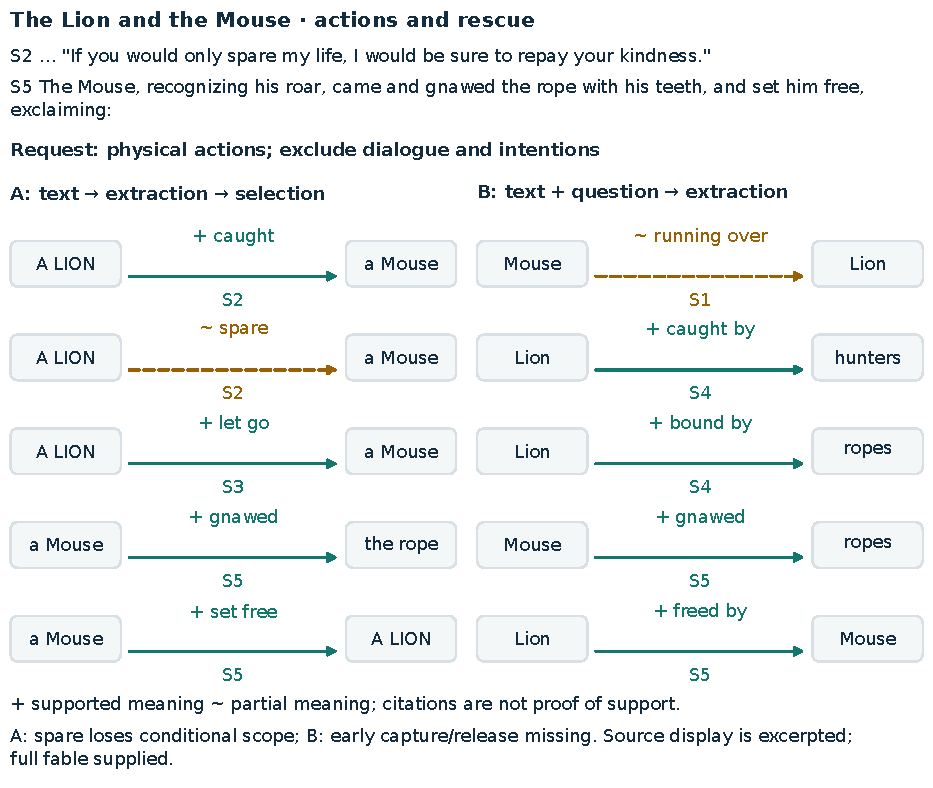
\includegraphics[width=158.0134mm]{figures/fable.pdf}\end{center}

\begin{center}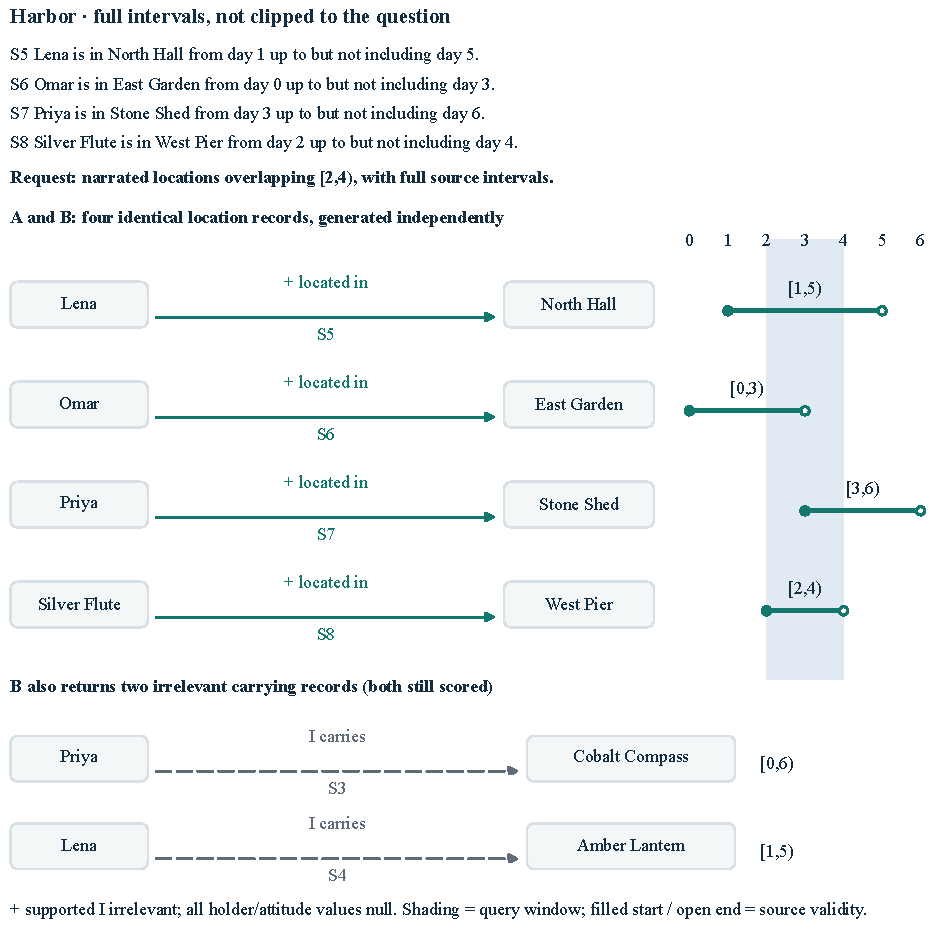
\includegraphics[width=158.0134mm]{figures/harbor.pdf}\end{center}

\begin{center}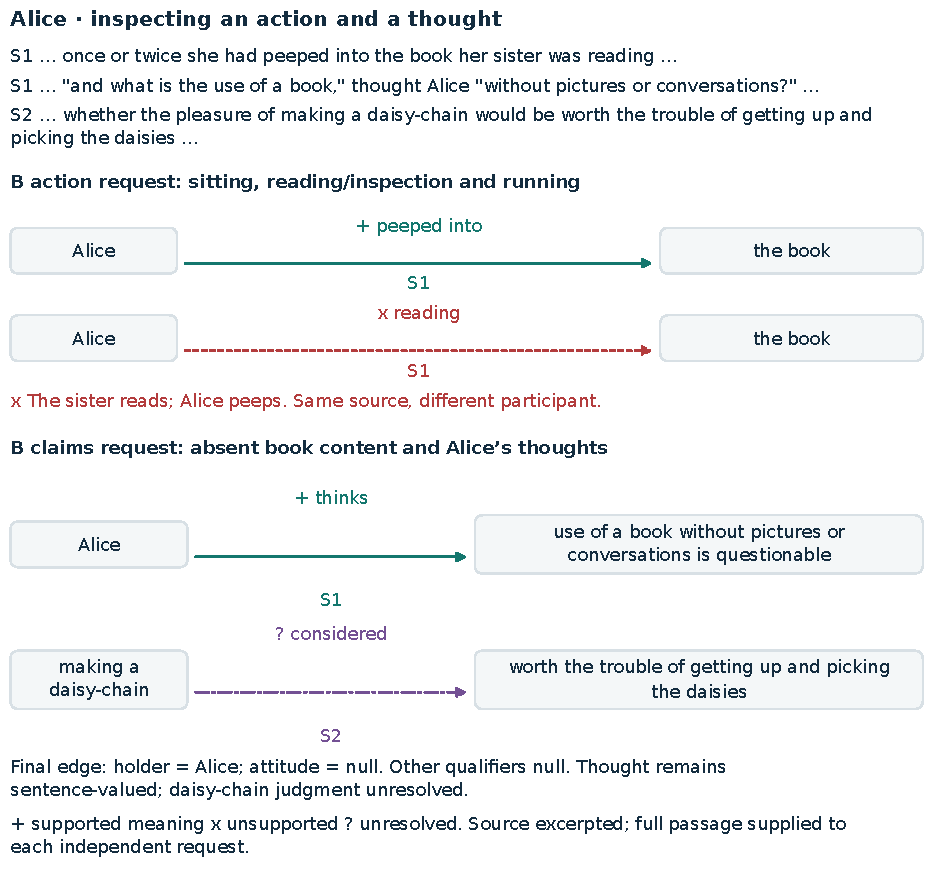
\includegraphics[width=158.0134mm]{figures/alice.pdf}\end{center}

\clearpage\section*{Compact Stories v2}

\subsection*{Common System Message (Exact Content)}

\VerbatimInput[fontsize=\small,breaklines=true,breakanywhere=true]{data/compact_system_message.txt}

\subsection*{Generation Settings}

\{"best\_of": 1, "chat\_template\_kwargs": \{"enable\_thinking": false\}, "frequency\_penalty": 0.0, "ignore\_eos": false, "max\_tokens": 2048, "min\_p": 0.0, "model": "qwen3-8b-awq-fallback", "n": 1, "presence\_penalty": 0.0, "repetition\_penalty": 1.0, "seed": 1988649846, "stop\_token\_ids": [151645], "stream": true, "stream\_options": \{"continuous\_usage\_stats": false, "include\_usage": true\}, "temperature": 0.7, "top\_k": 20, "top\_p": 0.8, "use\_beam\_search": false\}

Input is the pinned Qwen template, nonthinking; maximum context 12,288, maximum output 2,048. Strict agreement uses one-to-one normalized matching of relationships, citation sets and qualifications. All predictions remain in denominators. A valid citation is not support. All frozen rules, including exact aliases, are provided in data/evaluation\_rules.json. The main paper reports strict F1 separately from semantic support and target coverage.

\clearpage\subsection*{The harbor supplies}

\subsubsection*{Complete Supplied Evidence}

\noindent\textbf{S1} Lena owns Cobalt Compass.\par\smallskip

\noindent\textbf{S2} Omar owns Amber Lantern.\par\smallskip

\noindent\textbf{S3} Priya carries Cobalt Compass from day 0 up to but not including day 6.\par\smallskip

\noindent\textbf{S4} Lena carries Amber Lantern from day 1 up to but not including day 5.\par\smallskip

\noindent\textbf{S5} Lena is in North Hall from day 1 up to but not including day 5.\par\smallskip

\noindent\textbf{S6} Omar is in East Garden from day 0 up to but not including day 3.\par\smallskip

\noindent\textbf{S7} Priya is in Stone Shed from day 3 up to but not including day 6.\par\smallskip

\noindent\textbf{S8} Silver Flute is in West Pier from day 2 up to but not including day 4.\par\smallskip

\noindent\textbf{S9} Lena believes that Cobalt Compass is in North Hall.\par\smallskip

\noindent\textbf{S10} In reality, Cobalt Compass is in East Garden.\par\smallskip

\noindent\textbf{S11} Omar believes that Amber Lantern is in Stone Shed.\par\smallskip

\noindent\textbf{S12} In reality, Amber Lantern is in West Pier.\par\smallskip

\noindent\textbf{S13} Priya owns Silver Flute.\par\smallskip

\noindent\textbf{S14} Lena is in Stone Shed from day 7 up to but not including day 9.\par\smallskip

\subsubsection*{A pre-extract/select / possession}

\noindent\textbf{Exact question:} Who owns or carries what? Return all and only directly narrated ownership and carrying relationships, retaining every stated interval.\par

\noindent\textbf{Assessment:} Parseable: True; finish reason: stop.

Qualified matches 5/5 predictions, 5 targets; P/R/F1 (rounded) 1.000/1.000/1.000.\par

Actual output: call 1. The records are printed in full in the retained-calls section below. Selected-view record mapping (one-based):

View record 1: source record(s) 1\par

View record 2: source record(s) 2\par

View record 3: source record(s) 3\par

View record 4: source record(s) 4\par

View record 5: source record(s) 13\par

Record 1: correct\_complete\_fact; valid citation True; temporal True; epistemic True; issues []\par

Record 2: correct\_complete\_fact; valid citation True; temporal True; epistemic True; issues []\par

Record 3: correct\_complete\_fact; valid citation True; temporal True; epistemic True; issues []\par

Record 4: correct\_complete\_fact; valid citation True; temporal True; epistemic True; issues []\par

Record 5: correct\_complete\_fact; valid citation True; temporal True; epistemic True; issues []\par

\subsubsection*{B contextual / possession}

\noindent\textbf{Exact question:} Who owns or carries what? Return all and only directly narrated ownership and carrying relationships, retaining every stated interval.\par

\noindent\textbf{Assessment:} Parseable: True; finish reason: stop.

Qualified matches 5/10 predictions, 5 targets; P/R/F1 (rounded) 0.500/1.000/0.667.\par

Actual output: call 4. The records are printed in full in the retained-calls section below. Selected-view record mapping (one-based):

View record 1: source record(s) 1\par

View record 2: source record(s) 2\par

View record 3: source record(s) 3\par

View record 4: source record(s) 4\par

View record 5: source record(s) 5\par

View record 6: source record(s) 6\par

View record 7: source record(s) 7\par

View record 8: source record(s) 8\par

View record 9: source record(s) 9\par

View record 10: source record(s) 10\par

Record 1: correct\_complete\_fact; valid citation True; temporal True; epistemic True; issues []\par

Record 2: correct\_complete\_fact; valid citation True; temporal True; epistemic True; issues []\par

Record 3: correct\_complete\_fact; valid citation True; temporal True; epistemic True; issues []\par

Record 4: correct\_complete\_fact; valid citation True; temporal True; epistemic True; issues []\par

Record 5: supported\_but\_irrelevant; valid citation True; temporal True; epistemic True; issues []\par

Record 6: correct\_complete\_fact; valid citation True; temporal True; epistemic True; issues []\par

Record 7: supported\_but\_irrelevant; valid citation True; temporal True; epistemic True; issues []\par

Record 8: supported\_but\_irrelevant; valid citation True; temporal True; epistemic True; issues []\par

Record 9: supported\_but\_irrelevant; valid citation True; temporal True; epistemic True; issues []\par

Record 10: supported\_but\_irrelevant; valid citation True; temporal True; epistemic True; issues []\par

\noindent\textbf{Reference alternatives for this question, shared by A and B (not model output):}

\noindent Alternative 1:

"Lena" | "owns" | "Cobalt Compass" | ["S1"] | null | null | null | null\par\smallskip

"Omar" | "owns" | "Amber Lantern" | ["S2"] | null | null | null | null\par\smallskip

"Priya" | "carries" | "Cobalt Compass" | ["S3"] | 0 | 6 | null | null\par\smallskip

"Lena" | "carries" | "Amber Lantern" | ["S4"] | 1 | 5 | null | null\par\smallskip

"Priya" | "owns" | "Silver Flute" | ["S13"] | null | null | null | null\par\smallskip

\subsubsection*{A pre-extract/select / locations}

\noindent\textbf{Exact question:} Which directly narrated location relationships have an explicitly stated interval overlapping day 2 up to but not including day 4? Return all of them with their full evidence-stated intervals, not clipped to the question window. Exclude undated locations and beliefs.\par

\noindent\textbf{Assessment:} Parseable: True; finish reason: stop.

Qualified matches 4/4 predictions, 4 targets; P/R/F1 (rounded) 1.000/1.000/1.000.\par

Actual output: call 1. The records are printed in full in the retained-calls section below. Selected-view record mapping (one-based):

View record 1: source record(s) 5\par

View record 2: source record(s) 6\par

View record 3: source record(s) 7\par

View record 4: source record(s) 8\par

Record 1: correct\_complete\_fact; valid citation True; temporal True; epistemic True; issues []\par

Record 2: correct\_complete\_fact; valid citation True; temporal True; epistemic True; issues []\par

Record 3: correct\_complete\_fact; valid citation True; temporal True; epistemic True; issues []\par

Record 4: correct\_complete\_fact; valid citation True; temporal True; epistemic True; issues []\par

\subsubsection*{B contextual / locations}

\noindent\textbf{Exact question:} Which directly narrated location relationships have an explicitly stated interval overlapping day 2 up to but not including day 4? Return all of them with their full evidence-stated intervals, not clipped to the question window. Exclude undated locations and beliefs.\par

\noindent\textbf{Assessment:} Parseable: True; finish reason: stop.

Qualified matches 4/6 predictions, 4 targets; P/R/F1 (rounded) 0.667/1.000/0.800.\par

Actual output: call 5. The records are printed in full in the retained-calls section below. Selected-view record mapping (one-based):

View record 1: source record(s) 1\par

View record 2: source record(s) 2\par

View record 3: source record(s) 3\par

View record 4: source record(s) 4\par

View record 5: source record(s) 5\par

View record 6: source record(s) 6\par

Record 1: supported\_but\_irrelevant; valid citation True; temporal True; epistemic True; issues []\par

Record 2: supported\_but\_irrelevant; valid citation True; temporal True; epistemic True; issues []\par

Record 3: correct\_complete\_fact; valid citation True; temporal True; epistemic True; issues []\par

Record 4: correct\_complete\_fact; valid citation True; temporal True; epistemic True; issues []\par

Record 5: correct\_complete\_fact; valid citation True; temporal True; epistemic True; issues []\par

Record 6: correct\_complete\_fact; valid citation True; temporal True; epistemic True; issues []\par

\noindent\textbf{Reference alternatives for this question, shared by A and B (not model output):}

\noindent Alternative 1:

"Lena" | "located\_in" | "North Hall" | ["S5"] | 1 | 5 | null | null\par\smallskip

"Omar" | "located\_in" | "East Garden" | ["S6"] | 0 | 3 | null | null\par\smallskip

"Priya" | "located\_in" | "Stone Shed" | ["S7"] | 3 | 6 | null | null\par\smallskip

"Silver Flute" | "located\_in" | "West Pier" | ["S8"] | 2 | 4 | null | null\par\smallskip

\subsubsection*{A pre-extract/select / belief}

\noindent\textbf{Exact question:} Who explicitly believes what, and what reality is separately narrated about those same objects? Return each underlying believed relationship with its attribution and each matching narrated reality without attribution. Omit unrelated facts.\par

\noindent\textbf{Assessment:} Parseable: True; finish reason: stop.

Qualified matches 0/5 predictions, 4 targets; P/R/F1 (rounded) 0.000/0.000/0.000.\par

Actual output: call 1. The records are printed in full in the retained-calls section below. Selected-view record mapping (one-based):

View record 1: source record(s) 5\par

View record 2: source record(s) 6\par

View record 3: source record(s) 9\par

View record 4: source record(s) 11\par

View record 5: source record(s) 14\par

Record 1: supported\_but\_irrelevant; valid citation True; temporal True; epistemic True; issues []\par

Record 2: supported\_but\_irrelevant; valid citation True; temporal True; epistemic True; issues []\par

Record 3: unresolved\_wording; valid citation True; temporal None; epistemic None; issues ["holder and attitude must appear together"]\par

Record 4: unresolved\_wording; valid citation True; temporal None; epistemic None; issues ["holder and attitude must appear together"]\par

Record 5: supported\_but\_irrelevant; valid citation True; temporal True; epistemic True; issues []\par

\subsubsection*{B contextual / belief}

\noindent\textbf{Exact question:} Who explicitly believes what, and what reality is separately narrated about those same objects? Return each underlying believed relationship with its attribution and each matching narrated reality without attribution. Omit unrelated facts.\par

\noindent\textbf{Assessment:} Parseable: True; finish reason: stop.

Qualified matches 2/14 predictions, 4 targets; P/R/F1 (rounded) 0.143/0.500/0.222.\par

Actual output: call 6. The records are printed in full in the retained-calls section below. Selected-view record mapping (one-based):

View record 1: source record(s) 1\par

View record 2: source record(s) 2\par

View record 3: source record(s) 3\par

View record 4: source record(s) 4\par

View record 5: source record(s) 5\par

View record 6: source record(s) 6\par

View record 7: source record(s) 7\par

View record 8: source record(s) 8\par

View record 9: source record(s) 9\par

View record 10: source record(s) 10\par

View record 11: source record(s) 11\par

View record 12: source record(s) 12\par

View record 13: source record(s) 13\par

View record 14: source record(s) 14\par

Record 1: supported\_but\_irrelevant; valid citation True; temporal True; epistemic True; issues []\par

Record 2: supported\_but\_irrelevant; valid citation True; temporal True; epistemic True; issues []\par

Record 3: supported\_but\_irrelevant; valid citation True; temporal True; epistemic True; issues []\par

Record 4: supported\_but\_irrelevant; valid citation True; temporal True; epistemic True; issues []\par

Record 5: supported\_but\_irrelevant; valid citation True; temporal True; epistemic True; issues []\par

Record 6: supported\_but\_irrelevant; valid citation True; temporal True; epistemic True; issues []\par

Record 7: supported\_but\_irrelevant; valid citation True; temporal True; epistemic True; issues []\par

Record 8: supported\_but\_irrelevant; valid citation True; temporal True; epistemic True; issues []\par

Record 9: supported\_but\_irrelevant; valid citation True; temporal True; epistemic True; issues []\par

Record 10: unresolved\_wording; valid citation True; temporal None; epistemic None; issues []\par

Record 11: correct\_complete\_fact; valid citation True; temporal True; epistemic True; issues []\par

Record 12: unresolved\_wording; valid citation True; temporal None; epistemic None; issues []\par

Record 13: correct\_complete\_fact; valid citation True; temporal True; epistemic True; issues []\par

Record 14: supported\_but\_irrelevant; valid citation True; temporal True; epistemic True; issues []\par

\noindent\textbf{Reference alternatives for this question, shared by A and B (not model output):}

\noindent Alternative 1:

"Cobalt Compass" | "located\_in" | "North Hall" | ["S9"] | null | null | "Lena" | "believes"\par\smallskip

"Cobalt Compass" | "located\_in" | "East Garden" | ["S10"] | null | null | null | null\par\smallskip

"Amber Lantern" | "located\_in" | "Stone Shed" | ["S11"] | null | null | "Omar" | "believes"\par\smallskip

"Amber Lantern" | "located\_in" | "West Pier" | ["S12"] | null | null | null | null\par\smallskip

\subsubsection*{Retained Calls: Exact Tasks and Complete Output Records}

\subsubsection*{Call 1}

Input/output tokens: 660/605; request seconds 10.943192922510207; finish stop.

\noindent\textbf{Exact task (insert in the printed wrapper with this complete source):}\par Extract every explicitly stated relationship in all supplied sentences, including each belief and separately narrated reality. Retain all explicitly stated intervals. Do not infer additional relationships.

\noindent\textbf{1.} "Lena" | "owns" | "Cobalt Compass" | ["S1"] | null | null | null | null\par\smallskip

\noindent\textbf{2.} "Omar" | "owns" | "Amber Lantern" | ["S2"] | null | null | null | null\par\smallskip

\noindent\textbf{3.} "Priya" | "carries" | "Cobalt Compass" | ["S3"] | 0 | 6 | null | null\par\smallskip

\noindent\textbf{4.} "Lena" | "carries" | "Amber Lantern" | ["S4"] | 1 | 5 | null | null\par\smallskip

\noindent\textbf{5.} "Lena" | "located\_in" | "North Hall" | ["S5"] | 1 | 5 | null | null\par\smallskip

\noindent\textbf{6.} "Omar" | "located\_in" | "East Garden" | ["S6"] | 0 | 3 | null | null\par\smallskip

\noindent\textbf{7.} "Priya" | "located\_in" | "Stone Shed" | ["S7"] | 3 | 6 | null | null\par\smallskip

\noindent\textbf{8.} "Silver Flute" | "located\_in" | "West Pier" | ["S8"] | 2 | 4 | null | null\par\smallskip

\noindent\textbf{9.} "Lena" | "believes" | "Cobalt Compass is in North Hall" | ["S9"] | null | null | null | "believes"\par\smallskip

\noindent\textbf{10.} "Cobalt Compass" | "located\_in" | "East Garden" | ["S10"] | null | null | null | null\par\smallskip

\noindent\textbf{11.} "Omar" | "believes" | "Amber Lantern is in Stone Shed" | ["S11"] | null | null | null | "believes"\par\smallskip

\noindent\textbf{12.} "Amber Lantern" | "located\_in" | "West Pier" | ["S12"] | null | null | null | null\par\smallskip

\noindent\textbf{13.} "Priya" | "owns" | "Silver Flute" | ["S13"] | null | null | null | null\par\smallskip

\noindent\textbf{14.} "Lena" | "located\_in" | "Stone Shed" | ["S14"] | 7 | 9 | null | null\par\smallskip

\subsubsection*{Call 4}

Input/output tokens: 651/422; request seconds 7.605403192341328; finish stop.

\noindent\textbf{Exact task (insert in the printed wrapper with this complete source):}\par Who owns or carries what? Return all and only directly narrated ownership and carrying relationships, retaining every stated interval.

\noindent\textbf{1.} "Lena" | "owns" | "Cobalt Compass" | ["S1"] | null | null | null | null\par\smallskip

\noindent\textbf{2.} "Omar" | "owns" | "Amber Lantern" | ["S2"] | null | null | null | null\par\smallskip

\noindent\textbf{3.} "Priya" | "carries" | "Cobalt Compass" | ["S3"] | 0 | 6 | null | null\par\smallskip

\noindent\textbf{4.} "Lena" | "carries" | "Amber Lantern" | ["S4"] | 1 | 5 | null | null\par\smallskip

\noindent\textbf{5.} "Silver Flute" | "located\_in" | "West Pier" | ["S8"] | 2 | 4 | null | null\par\smallskip

\noindent\textbf{6.} "Priya" | "owns" | "Silver Flute" | ["S13"] | null | null | null | null\par\smallskip

\noindent\textbf{7.} "Lena" | "is\_in" | "North Hall" | ["S5"] | 1 | 5 | null | null\par\smallskip

\noindent\textbf{8.} "Omar" | "is\_in" | "East Garden" | ["S6"] | 0 | 3 | null | null\par\smallskip

\noindent\textbf{9.} "Priya" | "is\_in" | "Stone Shed" | ["S7"] | 3 | 6 | null | null\par\smallskip

\noindent\textbf{10.} "Lena" | "is\_in" | "Stone Shed" | ["S14"] | 7 | 9 | null | null\par\smallskip

\subsubsection*{Call 5}

Input/output tokens: 678/255; request seconds 5.284503255970776; finish stop.

\noindent\textbf{Exact task (insert in the printed wrapper with this complete source):}\par Which directly narrated location relationships have an explicitly stated interval overlapping day 2 up to but not including day 4? Return all of them with their full evidence-stated intervals, not clipped to the question window. Exclude undated locations and beliefs.

\noindent\textbf{1.} "Priya" | "carries" | "Cobalt Compass" | ["S3"] | 0 | 6 | null | null\par\smallskip

\noindent\textbf{2.} "Lena" | "carries" | "Amber Lantern" | ["S4"] | 1 | 5 | null | null\par\smallskip

\noindent\textbf{3.} "Lena" | "located\_in" | "North Hall" | ["S5"] | 1 | 5 | null | null\par\smallskip

\noindent\textbf{4.} "Omar" | "located\_in" | "East Garden" | ["S6"] | 0 | 3 | null | null\par\smallskip

\noindent\textbf{5.} "Priya" | "located\_in" | "Stone Shed" | ["S7"] | 3 | 6 | null | null\par\smallskip

\noindent\textbf{6.} "Silver Flute" | "located\_in" | "West Pier" | ["S8"] | 2 | 4 | null | null\par\smallskip

\subsubsection*{Call 6}

Input/output tokens: 667/607; request seconds 10.842662897892296; finish stop.

\noindent\textbf{Exact task (insert in the printed wrapper with this complete source):}\par Who explicitly believes what, and what reality is separately narrated about those same objects? Return each underlying believed relationship with its attribution and each matching narrated reality without attribution. Omit unrelated facts.

\noindent\textbf{1.} "Lena" | "owns" | "Cobalt Compass" | ["S1"] | null | null | null | null\par\smallskip

\noindent\textbf{2.} "Omar" | "owns" | "Amber Lantern" | ["S2"] | null | null | null | null\par\smallskip

\noindent\textbf{3.} "Priya" | "carries" | "Cobalt Compass" | ["S3"] | 0 | 6 | null | null\par\smallskip

\noindent\textbf{4.} "Lena" | "carries" | "Amber Lantern" | ["S4"] | 1 | 5 | null | null\par\smallskip

\noindent\textbf{5.} "Lena" | "located\_in" | "North Hall" | ["S5"] | 1 | 5 | null | null\par\smallskip

\noindent\textbf{6.} "Omar" | "located\_in" | "East Garden" | ["S6"] | 0 | 3 | null | null\par\smallskip

\noindent\textbf{7.} "Priya" | "located\_in" | "Stone Shed" | ["S7"] | 3 | 6 | null | null\par\smallskip

\noindent\textbf{8.} "Silver Flute" | "located\_in" | "West Pier" | ["S8"] | 2 | 4 | null | null\par\smallskip

\noindent\textbf{9.} "Priya" | "owns" | "Silver Flute" | ["S13"] | null | null | null | null\par\smallskip

\noindent\textbf{10.} "Lena" | "believes" | "Cobalt Compass is in North Hall" | ["S9"] | null | null | "Lena" | "believes"\par\smallskip

\noindent\textbf{11.} "Cobalt Compass" | "located\_in" | "East Garden" | ["S10"] | null | null | null | null\par\smallskip

\noindent\textbf{12.} "Omar" | "believes" | "Amber Lantern is in Stone Shed" | ["S11"] | null | null | "Omar" | "believes"\par\smallskip

\noindent\textbf{13.} "Amber Lantern" | "located\_in" | "West Pier" | ["S12"] | null | null | null | null\par\smallskip

\noindent\textbf{14.} "Lena" | "located\_in" | "Stone Shed" | ["S14"] | 7 | 9 | null | null\par\smallskip

\clearpage\subsection*{Museum preparations}

\subsubsection*{Complete Supplied Evidence}

\noindent\textbf{S1} Niko believes that Pearl Box is in Glass Room.\par\smallskip

\noindent\textbf{S2} Esme owns Ruby Medal.\par\smallskip

\noindent\textbf{S3} Dario is in Upper Court from day 20 up to but not including day 23.\par\smallskip

\noindent\textbf{S4} In reality, Pearl Box is in Brick Store.\par\smallskip

\noindent\textbf{S5} Niko carries Ruby Medal from day 19 up to but not including day 26.\par\smallskip

\noindent\textbf{S6} Onyx Bell is in Cedar Gate from day 23 up to but not including day 27.\par\smallskip

\noindent\textbf{S7} Esme believes that Ruby Medal is in Cedar Gate.\par\smallskip

\noindent\textbf{S8} Dario owns Onyx Bell.\par\smallskip

\noindent\textbf{S9} Esme is in Glass Room from day 21 up to but not including day 25.\par\smallskip

\noindent\textbf{S10} In reality, Ruby Medal is in Upper Court.\par\smallskip

\noindent\textbf{S11} Niko owns Pearl Box.\par\smallskip

\noindent\textbf{S12} Niko is in Brick Store from day 24 up to but not including day 28.\par\smallskip

\noindent\textbf{S13} Esme carries Pearl Box from day 20 up to but not including day 24.\par\smallskip

\noindent\textbf{S14} Dario is in Cedar Gate from day 28 up to but not including day 30.\par\smallskip

\subsubsection*{A pre-extract/select / possession}

\noindent\textbf{Exact question:} Who owns or carries what? Return all and only directly narrated ownership and carrying relationships, retaining every stated interval.\par

\noindent\textbf{Assessment:} Parseable: True; finish reason: stop.

Qualified matches 5/5 predictions, 5 targets; P/R/F1 (rounded) 1.000/1.000/1.000.\par

Actual output: call 3. The records are printed in full in the retained-calls section below. Selected-view record mapping (one-based):

View record 1: source record(s) 2\par

View record 2: source record(s) 5\par

View record 3: source record(s) 10\par

View record 4: source record(s) 12\par

View record 5: source record(s) 13\par

Record 1: correct\_complete\_fact; valid citation True; temporal True; epistemic True; issues []\par

Record 2: correct\_complete\_fact; valid citation True; temporal True; epistemic True; issues []\par

Record 3: correct\_complete\_fact; valid citation True; temporal True; epistemic True; issues []\par

Record 4: correct\_complete\_fact; valid citation True; temporal True; epistemic True; issues []\par

Record 5: correct\_complete\_fact; valid citation True; temporal True; epistemic True; issues []\par

\subsubsection*{B contextual / possession}

\noindent\textbf{Exact question:} Who owns or carries what? Return all and only directly narrated ownership and carrying relationships, retaining every stated interval.\par

\noindent\textbf{Assessment:} Parseable: True; finish reason: stop.

Qualified matches 5/13 predictions, 5 targets; P/R/F1 (rounded) 0.385/1.000/0.556.\par

Actual output: call 10. The records are printed in full in the retained-calls section below. Selected-view record mapping (one-based):

View record 1: source record(s) 1\par

View record 2: source record(s) 2\par

View record 3: source record(s) 3\par

View record 4: source record(s) 4\par

View record 5: source record(s) 5\par

View record 6: source record(s) 6\par

View record 7: source record(s) 7\par

View record 8: source record(s) 8\par

View record 9: source record(s) 9\par

View record 10: source record(s) 10\par

View record 11: source record(s) 11\par

View record 12: source record(s) 12\par

View record 13: source record(s) 13\par

Record 1: unresolved\_wording; valid citation True; temporal None; epistemic None; issues ["holder and attitude must appear together"]\par

Record 2: correct\_complete\_fact; valid citation True; temporal True; epistemic True; issues []\par

Record 3: supported\_but\_irrelevant; valid citation True; temporal True; epistemic True; issues []\par

Record 4: correct\_complete\_fact; valid citation True; temporal True; epistemic True; issues []\par

Record 5: supported\_but\_irrelevant; valid citation True; temporal True; epistemic True; issues []\par

Record 6: unresolved\_wording; valid citation True; temporal None; epistemic None; issues ["holder and attitude must appear together"]\par

Record 7: supported\_but\_irrelevant; valid citation True; temporal True; epistemic True; issues []\par

Record 8: supported\_but\_irrelevant; valid citation True; temporal True; epistemic True; issues []\par

Record 9: correct\_complete\_fact; valid citation True; temporal True; epistemic True; issues []\par

Record 10: correct\_complete\_fact; valid citation True; temporal True; epistemic True; issues []\par

Record 11: supported\_but\_irrelevant; valid citation True; temporal True; epistemic True; issues []\par

Record 12: supported\_but\_irrelevant; valid citation True; temporal True; epistemic True; issues []\par

Record 13: correct\_complete\_fact; valid citation True; temporal True; epistemic True; issues []\par

\noindent\textbf{Reference alternatives for this question, shared by A and B (not model output):}

\noindent Alternative 1:

"Esme" | "owns" | "Ruby Medal" | ["S2"] | null | null | null | null\par\smallskip

"Niko" | "carries" | "Ruby Medal" | ["S5"] | 19 | 26 | null | null\par\smallskip

"Dario" | "owns" | "Onyx Bell" | ["S8"] | null | null | null | null\par\smallskip

"Niko" | "owns" | "Pearl Box" | ["S11"] | null | null | null | null\par\smallskip

"Esme" | "carries" | "Pearl Box" | ["S13"] | 20 | 24 | null | null\par\smallskip

\subsubsection*{A pre-extract/select / locations}

\noindent\textbf{Exact question:} Which directly narrated location relationships have an explicitly stated interval overlapping day 22 up to but not including day 25? Return all of them with their full evidence-stated intervals, not clipped to the question window. Exclude undated locations and beliefs.\par

\noindent\textbf{Assessment:} Parseable: True; finish reason: stop.

Qualified matches 4/4 predictions, 4 targets; P/R/F1 (rounded) 1.000/1.000/1.000.\par

Actual output: call 3. The records are printed in full in the retained-calls section below. Selected-view record mapping (one-based):

View record 1: source record(s) 3\par

View record 2: source record(s) 6\par

View record 3: source record(s) 8\par

View record 4: source record(s) 11\par

Record 1: correct\_complete\_fact; valid citation True; temporal True; epistemic True; issues []\par

Record 2: correct\_complete\_fact; valid citation True; temporal True; epistemic True; issues []\par

Record 3: correct\_complete\_fact; valid citation True; temporal True; epistemic True; issues []\par

Record 4: correct\_complete\_fact; valid citation True; temporal True; epistemic True; issues []\par

\subsubsection*{B contextual / locations}

\noindent\textbf{Exact question:} Which directly narrated location relationships have an explicitly stated interval overlapping day 22 up to but not including day 25? Return all of them with their full evidence-stated intervals, not clipped to the question window. Exclude undated locations and beliefs.\par

\noindent\textbf{Assessment:} Parseable: True; finish reason: stop.

Qualified matches 4/5 predictions, 4 targets; P/R/F1 (rounded) 0.800/1.000/0.889.\par

Actual output: call 11. The records are printed in full in the retained-calls section below. Selected-view record mapping (one-based):

View record 1: source record(s) 1\par

View record 2: source record(s) 2\par

View record 3: source record(s) 3\par

View record 4: source record(s) 4\par

View record 5: source record(s) 5\par

Record 1: correct\_complete\_fact; valid citation True; temporal True; epistemic True; issues []\par

Record 2: correct\_complete\_fact; valid citation True; temporal True; epistemic True; issues []\par

Record 3: correct\_complete\_fact; valid citation True; temporal True; epistemic True; issues []\par

Record 4: correct\_complete\_fact; valid citation True; temporal True; epistemic True; issues []\par

Record 5: supported\_but\_irrelevant; valid citation True; temporal True; epistemic True; issues []\par

\noindent\textbf{Reference alternatives for this question, shared by A and B (not model output):}

\noindent Alternative 1:

"Dario" | "located\_in" | "Upper Court" | ["S3"] | 20 | 23 | null | null\par\smallskip

"Onyx Bell" | "located\_in" | "Cedar Gate" | ["S6"] | 23 | 27 | null | null\par\smallskip

"Esme" | "located\_in" | "Glass Room" | ["S9"] | 21 | 25 | null | null\par\smallskip

"Niko" | "located\_in" | "Brick Store" | ["S12"] | 24 | 28 | null | null\par\smallskip

\subsubsection*{A pre-extract/select / belief}

\noindent\textbf{Exact question:} Who explicitly believes what, and what reality is separately narrated about those same objects? Return each underlying believed relationship with its attribution and each matching narrated reality without attribution. Omit unrelated facts.\par

\noindent\textbf{Assessment:} Parseable: True; finish reason: stop.

Qualified matches 0/4 predictions, 4 targets; P/R/F1 (rounded) 0.000/0.000/0.000.\par

Actual output: call 3. The records are printed in full in the retained-calls section below. Selected-view record mapping (one-based):

View record 1: source record(s) 1\par

View record 2: source record(s) 7\par

View record 3: source record(s) 8\par

View record 4: source record(s) 11\par

Record 1: unresolved\_wording; valid citation True; temporal None; epistemic None; issues ["holder and attitude must appear together"]\par

Record 2: unresolved\_wording; valid citation True; temporal None; epistemic None; issues ["holder and attitude must appear together"]\par

Record 3: supported\_but\_irrelevant; valid citation True; temporal True; epistemic True; issues []\par

Record 4: supported\_but\_irrelevant; valid citation True; temporal True; epistemic True; issues []\par

\subsubsection*{B contextual / belief}

\noindent\textbf{Exact question:} Who explicitly believes what, and what reality is separately narrated about those same objects? Return each underlying believed relationship with its attribution and each matching narrated reality without attribution. Omit unrelated facts.\par

\noindent\textbf{Assessment:} Parseable: True; finish reason: stop.

Qualified matches 2/14 predictions, 4 targets; P/R/F1 (rounded) 0.143/0.500/0.222.\par

Actual output: call 12. The records are printed in full in the retained-calls section below. Selected-view record mapping (one-based):

View record 1: source record(s) 1\par

View record 2: source record(s) 2\par

View record 3: source record(s) 3\par

View record 4: source record(s) 4\par

View record 5: source record(s) 5\par

View record 6: source record(s) 6\par

View record 7: source record(s) 7\par

View record 8: source record(s) 8\par

View record 9: source record(s) 9\par

View record 10: source record(s) 10\par

View record 11: source record(s) 11\par

View record 12: source record(s) 12\par

View record 13: source record(s) 13\par

View record 14: source record(s) 14\par

Record 1: unresolved\_wording; valid citation True; temporal None; epistemic None; issues ["holder and attitude must appear together"]\par

Record 2: correct\_complete\_fact; valid citation True; temporal True; epistemic True; issues []\par

Record 3: supported\_but\_irrelevant; valid citation True; temporal True; epistemic True; issues []\par

Record 4: supported\_but\_irrelevant; valid citation True; temporal True; epistemic True; issues []\par

Record 5: correct\_complete\_fact; valid citation True; temporal True; epistemic True; issues []\par

Record 6: unresolved\_wording; valid citation True; temporal None; epistemic None; issues ["holder and attitude must appear together"]\par

Record 7: supported\_but\_irrelevant; valid citation True; temporal True; epistemic True; issues []\par

Record 8: supported\_but\_irrelevant; valid citation True; temporal True; epistemic True; issues []\par

Record 9: supported\_but\_irrelevant; valid citation True; temporal True; epistemic True; issues []\par

Record 10: supported\_but\_irrelevant; valid citation True; temporal True; epistemic True; issues []\par

Record 11: supported\_but\_irrelevant; valid citation True; temporal True; epistemic True; issues []\par

Record 12: supported\_but\_irrelevant; valid citation True; temporal True; epistemic True; issues []\par

Record 13: supported\_but\_irrelevant; valid citation True; temporal True; epistemic True; issues []\par

Record 14: supported\_but\_irrelevant; valid citation True; temporal True; epistemic True; issues []\par

\noindent\textbf{Reference alternatives for this question, shared by A and B (not model output):}

\noindent Alternative 1:

"Pearl Box" | "located\_in" | "Glass Room" | ["S1"] | null | null | "Niko" | "believes"\par\smallskip

"Pearl Box" | "located\_in" | "Brick Store" | ["S4"] | null | null | null | null\par\smallskip

"Ruby Medal" | "located\_in" | "Cedar Gate" | ["S7"] | null | null | "Esme" | "believes"\par\smallskip

"Ruby Medal" | "located\_in" | "Upper Court" | ["S10"] | null | null | null | null\par\smallskip

\subsubsection*{Retained Calls: Exact Tasks and Complete Output Records}

\subsubsection*{Call 3}

Input/output tokens: 678/615; request seconds 10.758112357929349; finish stop.

\noindent\textbf{Exact task (insert in the printed wrapper with this complete source):}\par Extract every explicitly stated relationship in all supplied sentences, including each belief and separately narrated reality. Retain all explicitly stated intervals. Do not infer additional relationships.

\noindent\textbf{1.} "Niko" | "believes" | "Pearl Box is in Glass Room" | ["S1"] | null | null | null | "believes"\par\smallskip

\noindent\textbf{2.} "Esme" | "owns" | "Ruby Medal" | ["S2"] | null | null | null | null\par\smallskip

\noindent\textbf{3.} "Dario" | "is\_in" | "Upper Court" | ["S3"] | 20 | 23 | null | null\par\smallskip

\noindent\textbf{4.} "Pearl Box" | "located\_in" | "Brick Store" | ["S4"] | null | null | null | null\par\smallskip

\noindent\textbf{5.} "Niko" | "carries" | "Ruby Medal" | ["S5"] | 19 | 26 | null | null\par\smallskip

\noindent\textbf{6.} "Onyx Bell" | "located\_in" | "Cedar Gate" | ["S6"] | 23 | 27 | null | null\par\smallskip

\noindent\textbf{7.} "Esme" | "believes" | "Ruby Medal is in Cedar Gate" | ["S7"] | null | null | null | "believes"\par\smallskip

\noindent\textbf{8.} "Esme" | "is\_in" | "Glass Room" | ["S9"] | 21 | 25 | null | null\par\smallskip

\noindent\textbf{9.} "Ruby Medal" | "located\_in" | "Upper Court" | ["S10"] | null | null | null | null\par\smallskip

\noindent\textbf{10.} "Niko" | "owns" | "Pearl Box" | ["S11"] | null | null | null | null\par\smallskip

\noindent\textbf{11.} "Niko" | "is\_in" | "Brick Store" | ["S12"] | 24 | 28 | null | null\par\smallskip

\noindent\textbf{12.} "Esme" | "carries" | "Pearl Box" | ["S13"] | 20 | 24 | null | null\par\smallskip

\noindent\textbf{13.} "Dario" | "owns" | "Onyx Bell" | ["S8"] | null | null | null | null\par\smallskip

\noindent\textbf{14.} "Dario" | "is\_in" | "Cedar Gate" | ["S14"] | 28 | 30 | null | null\par\smallskip

\subsubsection*{Call 10}

Input/output tokens: 669/572; request seconds 9.410800637677312; finish stop.

\noindent\textbf{Exact task (insert in the printed wrapper with this complete source):}\par Who owns or carries what? Return all and only directly narrated ownership and carrying relationships, retaining every stated interval.

\noindent\textbf{1.} "Niko" | "believes" | "Pearl Box is in Glass Room" | ["S1"] | null | null | null | "believes"\par\smallskip

\noindent\textbf{2.} "Esme" | "owns" | "Ruby Medal" | ["S2"] | null | null | null | null\par\smallskip

\noindent\textbf{3.} "Dario" | "is in" | "Upper Court" | ["S3"] | 20 | 23 | null | null\par\smallskip

\noindent\textbf{4.} "Niko" | "carries" | "Ruby Medal" | ["S5"] | 19 | 26 | null | null\par\smallskip

\noindent\textbf{5.} "Onyx Bell" | "is in" | "Cedar Gate" | ["S6"] | 23 | 27 | null | null\par\smallskip

\noindent\textbf{6.} "Esme" | "believes" | "Ruby Medal is in Cedar Gate" | ["S7"] | null | null | null | "believes"\par\smallskip

\noindent\textbf{7.} "Esme" | "is in" | "Glass Room" | ["S9"] | 21 | 25 | null | null\par\smallskip

\noindent\textbf{8.} "Niko" | "is in" | "Brick Store" | ["S12"] | 24 | 28 | null | null\par\smallskip

\noindent\textbf{9.} "Esme" | "carries" | "Pearl Box" | ["S13"] | 20 | 24 | null | null\par\smallskip

\noindent\textbf{10.} "Dario" | "owns" | "Onyx Bell" | ["S8"] | null | null | null | null\par\smallskip

\noindent\textbf{11.} "Dario" | "is in" | "Cedar Gate" | ["S14"] | 28 | 30 | null | null\par\smallskip

\noindent\textbf{12.} "Ruby Medal" | "is in" | "Upper Court" | ["S10"] | null | null | null | null\par\smallskip

\noindent\textbf{13.} "Niko" | "owns" | "Pearl Box" | ["S11"] | null | null | null | null\par\smallskip

\subsubsection*{Call 11}

Input/output tokens: 698/226; request seconds 4.9330835016444325; finish stop.

\noindent\textbf{Exact task (insert in the printed wrapper with this complete source):}\par Which directly narrated location relationships have an explicitly stated interval overlapping day 22 up to but not including day 25? Return all of them with their full evidence-stated intervals, not clipped to the question window. Exclude undated locations and beliefs.

\noindent\textbf{1.} "Dario" | "located\_in" | "Upper Court" | ["S3"] | 20 | 23 | null | null\par\smallskip

\noindent\textbf{2.} "Onyx Bell" | "located\_in" | "Cedar Gate" | ["S6"] | 23 | 27 | null | null\par\smallskip

\noindent\textbf{3.} "Esme" | "located\_in" | "Glass Room" | ["S9"] | 21 | 25 | null | null\par\smallskip

\noindent\textbf{4.} "Niko" | "located\_in" | "Brick Store" | ["S12"] | 24 | 28 | null | null\par\smallskip

\noindent\textbf{5.} "Esme" | "carries" | "Pearl Box" | ["S13"] | 20 | 24 | null | null\par\smallskip

\subsubsection*{Call 12}

Input/output tokens: 685/615; request seconds 10.20686200261116; finish stop.

\noindent\textbf{Exact task (insert in the printed wrapper with this complete source):}\par Who explicitly believes what, and what reality is separately narrated about those same objects? Return each underlying believed relationship with its attribution and each matching narrated reality without attribution. Omit unrelated facts.

\noindent\textbf{1.} "Niko" | "believes" | "Pearl Box is in Glass Room" | ["S1"] | null | null | null | "believes"\par\smallskip

\noindent\textbf{2.} "Pearl Box" | "located\_in" | "Brick Store" | ["S4"] | null | null | null | null\par\smallskip

\noindent\textbf{3.} "Esme" | "owns" | "Ruby Medal" | ["S2"] | null | null | null | null\par\smallskip

\noindent\textbf{4.} "Niko" | "carries" | "Ruby Medal" | ["S5"] | 19 | 26 | null | null\par\smallskip

\noindent\textbf{5.} "Ruby Medal" | "located\_in" | "Upper Court" | ["S10"] | null | null | null | null\par\smallskip

\noindent\textbf{6.} "Esme" | "believes" | "Ruby Medal is in Cedar Gate" | ["S7"] | null | null | null | "believes"\par\smallskip

\noindent\textbf{7.} "Dario" | "is\_in" | "Upper Court" | ["S3"] | 20 | 23 | null | null\par\smallskip

\noindent\textbf{8.} "Onyx Bell" | "located\_in" | "Cedar Gate" | ["S6"] | 23 | 27 | null | null\par\smallskip

\noindent\textbf{9.} "Dario" | "owns" | "Onyx Bell" | ["S8"] | null | null | null | null\par\smallskip

\noindent\textbf{10.} "Esme" | "is\_in" | "Glass Room" | ["S9"] | 21 | 25 | null | null\par\smallskip

\noindent\textbf{11.} "Niko" | "owns" | "Pearl Box" | ["S11"] | null | null | null | null\par\smallskip

\noindent\textbf{12.} "Niko" | "is\_in" | "Brick Store" | ["S12"] | 24 | 28 | null | null\par\smallskip

\noindent\textbf{13.} "Esme" | "carries" | "Pearl Box" | ["S13"] | 20 | 24 | null | null\par\smallskip

\noindent\textbf{14.} "Dario" | "is\_in" | "Cedar Gate" | ["S14"] | 28 | 30 | null | null\par\smallskip

\clearpage\subsection*{The orchard delivery}

\subsubsection*{Complete Supplied Evidence}

\noindent\textbf{S1} Vera owns Copper Book.\par\smallskip

\noindent\textbf{S2} Soren owns Ivory Vase.\par\smallskip

\noindent\textbf{S3} Jun carries Copper Book from day 9 up to but not including day 17.\par\smallskip

\noindent\textbf{S4} Vera carries Ivory Vase from day 10 up to but not including day 16.\par\smallskip

\noindent\textbf{S5} Jun is in River Room from day 10 up to but not including day 14.\par\smallskip

\noindent\textbf{S6} Soren is in Hill Court from day 14 up to but not including day 18.\par\smallskip

\noindent\textbf{S7} Vera is in South Loft from day 11 up to but not including day 16.\par\smallskip

\noindent\textbf{S8} Jade Drum is in Elm Dock from day 12 up to but not including day 15.\par\smallskip

\noindent\textbf{S9} Soren believes that Copper Book is in South Loft.\par\smallskip

\noindent\textbf{S10} In reality, Copper Book is in River Room.\par\smallskip

\noindent\textbf{S11} Jun believes that Ivory Vase is in Hill Court.\par\smallskip

\noindent\textbf{S12} In reality, Ivory Vase is in Elm Dock.\par\smallskip

\noindent\textbf{S13} Jun owns Jade Drum.\par\smallskip

\noindent\textbf{S14} Jun is in South Loft from day 18 up to but not including day 20.\par\smallskip

\subsubsection*{A pre-extract/select / possession}

\noindent\textbf{Exact question:} Who owns or carries what? Return all and only directly narrated ownership and carrying relationships, retaining every stated interval.\par

\noindent\textbf{Assessment:} Parseable: True; finish reason: stop.

Qualified matches 5/5 predictions, 5 targets; P/R/F1 (rounded) 1.000/1.000/1.000.\par

Actual output: call 2. The records are printed in full in the retained-calls section below. Selected-view record mapping (one-based):

View record 1: source record(s) 1\par

View record 2: source record(s) 2\par

View record 3: source record(s) 3\par

View record 4: source record(s) 4\par

View record 5: source record(s) 13\par

Record 1: correct\_complete\_fact; valid citation True; temporal True; epistemic True; issues []\par

Record 2: correct\_complete\_fact; valid citation True; temporal True; epistemic True; issues []\par

Record 3: correct\_complete\_fact; valid citation True; temporal True; epistemic True; issues []\par

Record 4: correct\_complete\_fact; valid citation True; temporal True; epistemic True; issues []\par

Record 5: correct\_complete\_fact; valid citation True; temporal True; epistemic True; issues []\par

\subsubsection*{B contextual / possession}

\noindent\textbf{Exact question:} Who owns or carries what? Return all and only directly narrated ownership and carrying relationships, retaining every stated interval.\par

\noindent\textbf{Assessment:} Parseable: True; finish reason: stop.

Qualified matches 5/12 predictions, 5 targets; P/R/F1 (rounded) 0.417/1.000/0.588.\par

Actual output: call 7. The records are printed in full in the retained-calls section below. Selected-view record mapping (one-based):

View record 1: source record(s) 1\par

View record 2: source record(s) 2\par

View record 3: source record(s) 3\par

View record 4: source record(s) 4\par

View record 5: source record(s) 5\par

View record 6: source record(s) 6\par

View record 7: source record(s) 7\par

View record 8: source record(s) 8\par

View record 9: source record(s) 9\par

View record 10: source record(s) 10\par

View record 11: source record(s) 11\par

View record 12: source record(s) 12\par

Record 1: correct\_complete\_fact; valid citation True; temporal True; epistemic True; issues []\par

Record 2: correct\_complete\_fact; valid citation True; temporal True; epistemic True; issues []\par

Record 3: correct\_complete\_fact; valid citation True; temporal True; epistemic True; issues []\par

Record 4: correct\_complete\_fact; valid citation True; temporal True; epistemic True; issues []\par

Record 5: supported\_but\_irrelevant; valid citation True; temporal True; epistemic True; issues []\par

Record 6: supported\_but\_irrelevant; valid citation True; temporal True; epistemic True; issues []\par

Record 7: supported\_but\_irrelevant; valid citation True; temporal True; epistemic True; issues []\par

Record 8: supported\_but\_irrelevant; valid citation True; temporal True; epistemic True; issues []\par

Record 9: supported\_but\_irrelevant; valid citation True; temporal True; epistemic True; issues []\par

Record 10: supported\_but\_irrelevant; valid citation True; temporal True; epistemic True; issues []\par

Record 11: correct\_complete\_fact; valid citation True; temporal True; epistemic True; issues []\par

Record 12: supported\_but\_irrelevant; valid citation True; temporal True; epistemic True; issues []\par

\noindent\textbf{Reference alternatives for this question, shared by A and B (not model output):}

\noindent Alternative 1:

"Vera" | "owns" | "Copper Book" | ["S1"] | null | null | null | null\par\smallskip

"Soren" | "owns" | "Ivory Vase" | ["S2"] | null | null | null | null\par\smallskip

"Jun" | "carries" | "Copper Book" | ["S3"] | 9 | 17 | null | null\par\smallskip

"Vera" | "carries" | "Ivory Vase" | ["S4"] | 10 | 16 | null | null\par\smallskip

"Jun" | "owns" | "Jade Drum" | ["S13"] | null | null | null | null\par\smallskip

\subsubsection*{A pre-extract/select / locations}

\noindent\textbf{Exact question:} Which directly narrated location relationships have an explicitly stated interval overlapping day 12 up to but not including day 15? Return all of them with their full evidence-stated intervals, not clipped to the question window. Exclude undated locations and beliefs.\par

\noindent\textbf{Assessment:} Parseable: True; finish reason: stop.

Qualified matches 4/4 predictions, 4 targets; P/R/F1 (rounded) 1.000/1.000/1.000.\par

Actual output: call 2. The records are printed in full in the retained-calls section below. Selected-view record mapping (one-based):

View record 1: source record(s) 5\par

View record 2: source record(s) 6\par

View record 3: source record(s) 7\par

View record 4: source record(s) 8\par

Record 1: correct\_complete\_fact; valid citation True; temporal True; epistemic True; issues []\par

Record 2: correct\_complete\_fact; valid citation True; temporal True; epistemic True; issues []\par

Record 3: correct\_complete\_fact; valid citation True; temporal True; epistemic True; issues []\par

Record 4: correct\_complete\_fact; valid citation True; temporal True; epistemic True; issues []\par

\subsubsection*{B contextual / locations}

\noindent\textbf{Exact question:} Which directly narrated location relationships have an explicitly stated interval overlapping day 12 up to but not including day 15? Return all of them with their full evidence-stated intervals, not clipped to the question window. Exclude undated locations and beliefs.\par

\noindent\textbf{Assessment:} Parseable: True; finish reason: stop.

Qualified matches 3/5 predictions, 4 targets; P/R/F1 (rounded) 0.600/0.750/0.667.\par

Actual output: call 8. The records are printed in full in the retained-calls section below. Selected-view record mapping (one-based):

View record 1: source record(s) 1\par

View record 2: source record(s) 2\par

View record 3: source record(s) 3\par

View record 4: source record(s) 4\par

View record 5: source record(s) 5\par

Record 1: supported\_but\_irrelevant; valid citation True; temporal True; epistemic True; issues []\par

Record 2: supported\_but\_irrelevant; valid citation True; temporal True; epistemic True; issues []\par

Record 3: correct\_complete\_fact; valid citation True; temporal True; epistemic True; issues []\par

Record 4: correct\_complete\_fact; valid citation True; temporal True; epistemic True; issues []\par

Record 5: correct\_complete\_fact; valid citation True; temporal True; epistemic True; issues []\par

\noindent\textbf{Reference alternatives for this question, shared by A and B (not model output):}

\noindent Alternative 1:

"Jun" | "located\_in" | "River Room" | ["S5"] | 10 | 14 | null | null\par\smallskip

"Soren" | "located\_in" | "Hill Court" | ["S6"] | 14 | 18 | null | null\par\smallskip

"Vera" | "located\_in" | "South Loft" | ["S7"] | 11 | 16 | null | null\par\smallskip

"Jade Drum" | "located\_in" | "Elm Dock" | ["S8"] | 12 | 15 | null | null\par\smallskip

\subsubsection*{A pre-extract/select / belief}

\noindent\textbf{Exact question:} Who explicitly believes what, and what reality is separately narrated about those same objects? Return each underlying believed relationship with its attribution and each matching narrated reality without attribution. Omit unrelated facts.\par

\noindent\textbf{Assessment:} Parseable: True; finish reason: stop.

Qualified matches 4/4 predictions, 4 targets; P/R/F1 (rounded) 1.000/1.000/1.000.\par

Actual output: call 2. The records are printed in full in the retained-calls section below. Selected-view record mapping (one-based):

View record 1: source record(s) 9\par

View record 2: source record(s) 10\par

View record 3: source record(s) 11\par

View record 4: source record(s) 12\par

Record 1: correct\_complete\_fact; valid citation True; temporal True; epistemic True; issues []\par

Record 2: correct\_complete\_fact; valid citation True; temporal True; epistemic True; issues []\par

Record 3: correct\_complete\_fact; valid citation True; temporal True; epistemic True; issues []\par

Record 4: correct\_complete\_fact; valid citation True; temporal True; epistemic True; issues []\par

\subsubsection*{B contextual / belief}

\noindent\textbf{Exact question:} Who explicitly believes what, and what reality is separately narrated about those same objects? Return each underlying believed relationship with its attribution and each matching narrated reality without attribution. Omit unrelated facts.\par

\noindent\textbf{Assessment:} Parseable: True; finish reason: stop.

Qualified matches 2/13 predictions, 4 targets; P/R/F1 (rounded) 0.154/0.500/0.235.\par

Actual output: call 9. The records are printed in full in the retained-calls section below. Selected-view record mapping (one-based):

View record 1: source record(s) 1\par

View record 2: source record(s) 2\par

View record 3: source record(s) 3\par

View record 4: source record(s) 4\par

View record 5: source record(s) 5\par

View record 6: source record(s) 6\par

View record 7: source record(s) 7\par

View record 8: source record(s) 8\par

View record 9: source record(s) 9\par

View record 10: source record(s) 10\par

View record 11: source record(s) 11\par

View record 12: source record(s) 12\par

View record 13: source record(s) 13\par

Record 1: supported\_but\_irrelevant; valid citation True; temporal True; epistemic True; issues []\par

Record 2: supported\_but\_irrelevant; valid citation True; temporal True; epistemic True; issues []\par

Record 3: supported\_but\_irrelevant; valid citation True; temporal True; epistemic True; issues []\par

Record 4: supported\_but\_irrelevant; valid citation True; temporal True; epistemic True; issues []\par

Record 5: supported\_but\_irrelevant; valid citation True; temporal True; epistemic True; issues []\par

Record 6: supported\_but\_irrelevant; valid citation True; temporal True; epistemic True; issues []\par

Record 7: supported\_but\_irrelevant; valid citation True; temporal True; epistemic True; issues []\par

Record 8: unresolved\_wording; valid citation True; temporal None; epistemic None; issues []\par

Record 9: correct\_complete\_fact; valid citation True; temporal True; epistemic True; issues []\par

Record 10: unresolved\_wording; valid citation True; temporal None; epistemic None; issues []\par

Record 11: correct\_complete\_fact; valid citation True; temporal True; epistemic True; issues []\par

Record 12: supported\_but\_irrelevant; valid citation True; temporal True; epistemic True; issues []\par

Record 13: supported\_but\_irrelevant; valid citation True; temporal True; epistemic True; issues []\par

\noindent\textbf{Reference alternatives for this question, shared by A and B (not model output):}

\noindent Alternative 1:

"Copper Book" | "located\_in" | "South Loft" | ["S9"] | null | null | "Soren" | "believes"\par\smallskip

"Copper Book" | "located\_in" | "River Room" | ["S10"] | null | null | null | null\par\smallskip

"Ivory Vase" | "located\_in" | "Hill Court" | ["S11"] | null | null | "Jun" | "believes"\par\smallskip

"Ivory Vase" | "located\_in" | "Elm Dock" | ["S12"] | null | null | null | null\par\smallskip

\subsubsection*{Retained Calls: Exact Tasks and Complete Output Records}

\subsubsection*{Call 2}

Input/output tokens: 671/615; request seconds 10.896031664684415; finish stop.

\noindent\textbf{Exact task (insert in the printed wrapper with this complete source):}\par Extract every explicitly stated relationship in all supplied sentences, including each belief and separately narrated reality. Retain all explicitly stated intervals. Do not infer additional relationships.

\noindent\textbf{1.} "Vera" | "owns" | "Copper Book" | ["S1"] | null | null | null | null\par\smallskip

\noindent\textbf{2.} "Soren" | "owns" | "Ivory Vase" | ["S2"] | null | null | null | null\par\smallskip

\noindent\textbf{3.} "Jun" | "carries" | "Copper Book" | ["S3"] | 9 | 17 | null | null\par\smallskip

\noindent\textbf{4.} "Vera" | "carries" | "Ivory Vase" | ["S4"] | 10 | 16 | null | null\par\smallskip

\noindent\textbf{5.} "Jun" | "located\_in" | "River Room" | ["S5"] | 10 | 14 | null | null\par\smallskip

\noindent\textbf{6.} "Soren" | "located\_in" | "Hill Court" | ["S6"] | 14 | 18 | null | null\par\smallskip

\noindent\textbf{7.} "Vera" | "located\_in" | "South Loft" | ["S7"] | 11 | 16 | null | null\par\smallskip

\noindent\textbf{8.} "Jade Drum" | "located\_in" | "Elm Dock" | ["S8"] | 12 | 15 | null | null\par\smallskip

\noindent\textbf{9.} "Copper Book" | "located\_in" | "South Loft" | ["S9"] | null | null | "Soren" | "believes"\par\smallskip

\noindent\textbf{10.} "Copper Book" | "located\_in" | "River Room" | ["S10"] | null | null | null | null\par\smallskip

\noindent\textbf{11.} "Ivory Vase" | "located\_in" | "Hill Court" | ["S11"] | null | null | "Jun" | "believes"\par\smallskip

\noindent\textbf{12.} "Ivory Vase" | "located\_in" | "Elm Dock" | ["S12"] | null | null | null | null\par\smallskip

\noindent\textbf{13.} "Jun" | "owns" | "Jade Drum" | ["S13"] | null | null | null | null\par\smallskip

\noindent\textbf{14.} "Jun" | "located\_in" | "South Loft" | ["S14"] | 18 | 20 | null | null\par\smallskip

\subsubsection*{Call 7}

Input/output tokens: 662/524; request seconds 9.670006787404418; finish stop.

\noindent\textbf{Exact task (insert in the printed wrapper with this complete source):}\par Who owns or carries what? Return all and only directly narrated ownership and carrying relationships, retaining every stated interval.

\noindent\textbf{1.} "Vera" | "owns" | "Copper Book" | ["S1"] | null | null | null | null\par\smallskip

\noindent\textbf{2.} "Soren" | "owns" | "Ivory Vase" | ["S2"] | null | null | null | null\par\smallskip

\noindent\textbf{3.} "Jun" | "carries" | "Copper Book" | ["S3"] | 9 | 17 | null | null\par\smallskip

\noindent\textbf{4.} "Vera" | "carries" | "Ivory Vase" | ["S4"] | 10 | 16 | null | null\par\smallskip

\noindent\textbf{5.} "Jun" | "located\_in" | "River Room" | ["S5"] | 10 | 14 | null | null\par\smallskip

\noindent\textbf{6.} "Soren" | "located\_in" | "Hill Court" | ["S6"] | 14 | 18 | null | null\par\smallskip

\noindent\textbf{7.} "Vera" | "located\_in" | "South Loft" | ["S7"] | 11 | 16 | null | null\par\smallskip

\noindent\textbf{8.} "Jade Drum" | "located\_in" | "Elm Dock" | ["S8"] | 12 | 15 | null | null\par\smallskip

\noindent\textbf{9.} "Copper Book" | "located\_in" | "River Room" | ["S10"] | null | null | null | null\par\smallskip

\noindent\textbf{10.} "Ivory Vase" | "located\_in" | "Elm Dock" | ["S12"] | null | null | null | null\par\smallskip

\noindent\textbf{11.} "Jun" | "owns" | "Jade Drum" | ["S13"] | null | null | null | null\par\smallskip

\noindent\textbf{12.} "Jun" | "located\_in" | "South Loft" | ["S14"] | 18 | 20 | null | null\par\smallskip

\subsubsection*{Call 8}

Input/output tokens: 691/224; request seconds 4.735408819280565; finish stop.

\noindent\textbf{Exact task (insert in the printed wrapper with this complete source):}\par Which directly narrated location relationships have an explicitly stated interval overlapping day 12 up to but not including day 15? Return all of them with their full evidence-stated intervals, not clipped to the question window. Exclude undated locations and beliefs.

\noindent\textbf{1.} "Jun" | "carries" | "Copper Book" | ["S3"] | 9 | 17 | null | null\par\smallskip

\noindent\textbf{2.} "Vera" | "carries" | "Ivory Vase" | ["S4"] | 10 | 16 | null | null\par\smallskip

\noindent\textbf{3.} "Jun" | "located\_in" | "River Room" | ["S5"] | 10 | 14 | null | null\par\smallskip

\noindent\textbf{4.} "Soren" | "located\_in" | "Hill Court" | ["S6"] | 14 | 18 | null | null\par\smallskip

\noindent\textbf{5.} "Jade Drum" | "located\_in" | "Elm Dock" | ["S8"] | 12 | 15 | null | null\par\smallskip

\subsubsection*{Call 9}

Input/output tokens: 678/580; request seconds 9.434332771226764; finish stop.

\noindent\textbf{Exact task (insert in the printed wrapper with this complete source):}\par Who explicitly believes what, and what reality is separately narrated about those same objects? Return each underlying believed relationship with its attribution and each matching narrated reality without attribution. Omit unrelated facts.

\noindent\textbf{1.} "Soren" | "owns" | "Ivory Vase" | ["S2"] | null | null | null | null\par\smallskip

\noindent\textbf{2.} "Jun" | "carries" | "Copper Book" | ["S3"] | 9 | 17 | null | null\par\smallskip

\noindent\textbf{3.} "Vera" | "carries" | "Ivory Vase" | ["S4"] | 10 | 16 | null | null\par\smallskip

\noindent\textbf{4.} "Jun" | "located\_in" | "River Room" | ["S5"] | 10 | 14 | null | null\par\smallskip

\noindent\textbf{5.} "Soren" | "located\_in" | "Hill Court" | ["S6"] | 14 | 18 | null | null\par\smallskip

\noindent\textbf{6.} "Vera" | "located\_in" | "South Loft" | ["S7"] | 11 | 16 | null | null\par\smallskip

\noindent\textbf{7.} "Jade Drum" | "located\_in" | "Elm Dock" | ["S8"] | 12 | 15 | null | null\par\smallskip

\noindent\textbf{8.} "Soren" | "believes" | "Copper Book is in South Loft" | ["S9"] | null | null | "Soren" | "believes"\par\smallskip

\noindent\textbf{9.} "Copper Book" | "located\_in" | "River Room" | ["S10"] | null | null | null | null\par\smallskip

\noindent\textbf{10.} "Jun" | "believes" | "Ivory Vase is in Hill Court" | ["S11"] | null | null | "Jun" | "believes"\par\smallskip

\noindent\textbf{11.} "Ivory Vase" | "located\_in" | "Elm Dock" | ["S12"] | null | null | null | null\par\smallskip

\noindent\textbf{12.} "Jun" | "owns" | "Jade Drum" | ["S13"] | null | null | null | null\par\smallskip

\noindent\textbf{13.} "Jun" | "located\_in" | "South Loft" | ["S14"] | 18 | 20 | null | null\par\smallskip

\clearpage\section*{Published Prose}

\subsection*{Common System Message (Exact Content)}

\VerbatimInput[fontsize=\small,breaklines=true,breakanywhere=true]{data/prose_system_message.txt}

\subsection*{Generation Settings}

\{"best\_of": 1, "chat\_template\_kwargs": \{"enable\_thinking": false\}, "frequency\_penalty": 0.0, "ignore\_eos": false, "max\_tokens": 2048, "min\_p": 0.0, "model": "qwen3-8b-awq-fallback", "n": 1, "presence\_penalty": 0.0, "repetition\_penalty": 1.0, "seed": 1988649846, "stop\_token\_ids": [151645], "stream": true, "stream\_options": \{"continuous\_usage\_stats": false, "include\_usage": true\}, "temperature": 0.7, "top\_k": 20, "top\_p": 0.8, "use\_beam\_search": false\}

Input is the pinned Qwen template, nonthinking; maximum context 12,288, maximum output 2,048. Strict agreement uses one-to-one normalized matching of relationships, citation sets and qualifications. All predictions remain in denominators. A valid citation is not support. All frozen rules, including exact aliases, are provided in data/evaluation\_rules.json. The main paper reports strict F1 separately from semantic support and target coverage.

\clearpage\subsection*{Alice's Adventures in Wonderland}

\subsubsection*{Complete Supplied Evidence}

Lewis Carroll; translator: not applicable; Chapter I: Down the Rabbit-Hole, opening two paragraphs. \url{https://www.gutenberg.org/ebooks/11}. Retrieved 2026-09-09T13:42:39.616173+00:00. Project Gutenberg lists this edition as public domain in the USA; original attribution and complete supplied license notices retained. Check local law outside the USA.

\noindent\textbf{S1} Alice was beginning to get very tired of sitting by her sister on the
bank, and of having nothing to do: once or twice she had peeped into
the book her sister was reading, but it had no pictures or
conversations in it, ``and what is the use of a book,'' thought Alice
``without pictures or conversations?''\par\smallskip

\noindent\textbf{S2} 

So she was considering in her own mind (as well as she could, for the
hot day made her feel very sleepy and stupid), whether the pleasure of
making a daisy-chain would be worth the trouble of getting up and
picking the daisies, when suddenly a White Rabbit with pink eyes ran
close by her.\par\smallskip

\subsubsection*{A pre-extract/select / actions}

\noindent\textbf{Exact question:} Which sitting/location, reading/inspection and running relationships involve Alice, her sister, the book, bank and Rabbit? Exclude thoughts, feelings, appearance and book-content properties.\par

\noindent\textbf{Assessment:} Parseable: True; finish reason: stop.

Qualified matches 1/2 predictions, 5 targets; P/R/F1 (rounded) 0.500/0.200/0.286.\par

Actual output: call 2. The records are printed in full in the retained-calls section below. Selected-view record mapping (one-based):

View record 1: source record(s) 3\par

View record 2: source record(s) 8\par

\noindent Record 1: supported; qualifications correct; relevant True. S1 supports Alice peeping into the book; the model-authored object also explicitly says her sister was reading that book. Both meanings are present, though one is embedded in a long node label rather than a separate edge. This one record receives at most one supported-record credit and two distinct target-coverage credits.\par\smallskip

\noindent Record 2: supported; qualifications correct; relevant True. Frozen reference match, not independent verification.\par\smallskip

\subsubsection*{B contextual / actions}

\noindent\textbf{Exact question:} Which sitting/location, reading/inspection and running relationships involve Alice, her sister, the book, bank and Rabbit? Exclude thoughts, feelings, appearance and book-content properties.\par

\noindent\textbf{Assessment:} Parseable: True; finish reason: stop.

Qualified matches 2/5 predictions, 5 targets; P/R/F1 (rounded) 0.400/0.400/0.400.\par

Actual output: call 6. The records are printed in full in the retained-calls section below. Selected-view record mapping (one-based):

View record 1: source record(s) 1\par

View record 2: source record(s) 2\par

View record 3: source record(s) 3\par

View record 4: source record(s) 4\par

View record 5: source record(s) 5\par

\noindent Record 1: supported; qualifications correct; relevant True. Frozen reference match, not independent verification.\par\smallskip

\noindent Record 2: partial; qualifications correct; relevant True. S1 places Alice on the bank. sitting\_by bank instead expresses a coarser adjacent-location relationship, not the explicit on-bank target. Do not normalize the preposition away; partial spatial information only.\par\smallskip

\noindent Record 3: supported; qualifications correct; relevant True. Frozen reference match, not independent verification.\par\smallskip

\noindent Record 4: unsupported; qualifications correct; relevant True. S1 explicitly assigns reading to the sister and peeping to Alice. It does not support Alice reading the book. This is an unsupported participant/action assignment, not proof that Alice never read anything.\par\smallskip

\noindent Record 5: supported; qualifications correct; relevant True. S2 says the White Rabbit ran close by her, with her unambiguously Alice in the supplied passage. The output retains that exact referential phrase in its object. Manual meaning credit does not merge graph endpoints or change the strict matcher.\par\smallskip

\noindent\textbf{Reference alternatives for this question, shared by A and B (not model output):}

\noindent Alternative 1:

"Alice" | "sits\_by" | "Alice's sister" | ["S1"] | null | null | null | null\par\smallskip

"Alice" | "located\_on" | "bank" | ["S1"] | null | null | null | null\par\smallskip

"Alice's sister" | "reads" | "book" | ["S1"] | null | null | null | null\par\smallskip

"Alice" | "peeps\_into" | "book" | ["S1"] | null | null | null | null\par\smallskip

"White Rabbit" | "runs\_past" | "Alice" | ["S2"] | null | null | null | null\par\smallskip

\subsubsection*{A pre-extract/select / claims}

\noindent\textbf{Exact question:} What does the passage say about the book's absent content and Alice's thoughts about the usefulness of such books and making a daisy-chain? Exclude physical actions, locations, appearance and the Rabbit; preserve questions and consideration without treating them as decisions.\par

\noindent\textbf{Assessment:} Parseable: True; finish reason: stop.

Qualified matches 0/4 predictions, 4 targets; P/R/F1 (rounded) 0.000/0.000/0.000.\par

Actual output: call 2. The records are printed in full in the retained-calls section below. Selected-view record mapping (one-based):

View record 1: source record(s) 4\par

View record 2: source record(s) 5\par

View record 3: source record(s) 6\par

View record 4: source record(s) 7\par

\noindent Record 1: partial; qualifications correct; relevant True. This is an actual fragment of Alice's thought in S1. It drops the without-pictures-or-conversations restriction, so it does not independently preserve the full target. Do not join it to the next record to invent a complete proposition.\par\smallskip

\noindent Record 2: partial; qualifications unresolved; relevant True. The quoted words occur in S1, but 'without pictures or conversations' alone is not a proposition with a book referent or a question. Alice as thinker is explicit; complete qualification and meaning remain unresolved.\par\smallskip

\noindent Record 3: supported; qualifications correct; relevant True. S2 explicitly describes Alice considering the pleasure of making a daisy-chain. Consideration is retained rather than presented as a decision or completed act. The finer worth-versus-trouble deliberation is omitted; the frozen broad considers-making target is nevertheless explicit.\par\smallskip

\noindent Record 4: supported; qualifications correct; relevant True. S2 directly supports this fuller deliberation, including whether pleasure is worth the effort. It repeats the same broad target as the preceding record: semantic coverage counts that target once, and both predictions stay in strict denominators.\par\smallskip

\subsubsection*{B contextual / claims}

\noindent\textbf{Exact question:} What does the passage say about the book's absent content and Alice's thoughts about the usefulness of such books and making a daisy-chain? Exclude physical actions, locations, appearance and the Rabbit; preserve questions and consideration without treating them as decisions.\par

\noindent\textbf{Assessment:} Parseable: True; finish reason: stop.

Qualified matches 0/3 predictions, 4 targets; P/R/F1 (rounded) 0.000/0.000/0.000.\par

Actual output: call 7. The records are printed in full in the retained-calls section below. Selected-view record mapping (one-based):

View record 1: source record(s) 1\par

View record 2: source record(s) 2\par

View record 3: source record(s) 3\par

\noindent Record 1: supported; qualifications correct; relevant True. S1 explicitly says the book has no pictures or conversations. The combined negative object preserves both absent-content targets; one record receives one supported-record credit, and two unique semantic-coverage credits. No splitting or new model facts are performed.\par\smallskip

\noindent Record 2: supported; qualifications correct; relevant True. The subject Alice, mental predicate thinks, and object questioning the use of a pictureless/conversationless book preserve her rhetorical thought from S1. It is not asserted as objective uselessness. This semantically supported mental-act representation remains a strict wording mismatch.\par\smallskip

\noindent Record 3: unresolved; qualifications incorrect; relevant True. S2 says Alice is considering WHETHER making the chain would be worth the trouble. 'considered worth' may instead mean judged worthwhile. The missing attitude alongside holder Alice also violates the compact pairing rule. Source support for a settled positive judgment cannot be established; do not award the consideration target by guessing.\par\smallskip

\noindent\textbf{Reference alternatives for this question, shared by A and B (not model output):}

\noindent Alternative 1:

"book" | "lacks" | "pictures" | ["S1"] | null | null | null | null\par\smallskip

"book" | "lacks" | "conversations" | ["S1"] | null | null | null | null\par\smallskip

"Alice" | "questions\_usefulness\_of" | "book without pictures or conversations" | ["S1"] | null | null | null | null\par\smallskip

"Alice" | "considers\_making" | "daisy-chain" | ["S2"] | null | null | null | null\par\smallskip

\subsubsection*{Retained Calls: Exact Tasks and Complete Output Records}

\subsubsection*{Call 2}

Input/output tokens: 701/381; request seconds 7.268172011710703; finish stop.

\noindent\textbf{Exact task (insert in the printed wrapper with this complete source):}\par Extract the explicitly supported relationships throughout this complete excerpt. No contextual question is supplied; distinguish narration from attributed or uncertain content.

\noindent\textbf{1.} "Alice" | "is\_tired\_of" | "sitting by her sister on the bank" | ["S1"] | null | null | null | null\par\smallskip

\noindent\textbf{2.} "Alice" | "is\_tired\_of" | "having nothing to do" | ["S1"] | null | null | null | null\par\smallskip

\noindent\textbf{3.} "Alice" | "had\_peeped\_into" | "the book her sister was reading" | ["S1"] | null | null | null | null\par\smallskip

\noindent\textbf{4.} "Alice" | "thought" | "what is the use of a book" | ["S1"] | null | null | null | null\par\smallskip

\noindent\textbf{5.} "Alice" | "thought" | "without pictures or conversations" | ["S1"] | null | null | null | null\par\smallskip

\noindent\textbf{6.} "Alice" | "was\_considering" | "the pleasure of making a daisy-chain" | ["S2"] | null | null | null | null\par\smallskip

\noindent\textbf{7.} "Alice" | "was\_considering" | "whether the pleasure of making a daisy-chain would be worth the trouble of getting up and picking the daisies" | ["S2"] | null | null | null | null\par\smallskip

\noindent\textbf{8.} "White Rabbit" | "ran close by" | "Alice" | ["S2"] | null | null | null | null\par\smallskip

\subsubsection*{Call 6}

Input/output tokens: 711/208; request seconds 3.8374315928667784; finish stop.

\noindent\textbf{Exact task (insert in the printed wrapper with this complete source):}\par Which sitting/location, reading/inspection and running relationships involve Alice, her sister, the book, bank and Rabbit? Exclude thoughts, feelings, appearance and book-content properties.

\noindent\textbf{1.} "Alice" | "sitting\_by" | "her sister" | ["S1"] | null | null | null | null\par\smallskip

\noindent\textbf{2.} "Alice" | "sitting\_by" | "bank" | ["S1"] | null | null | null | null\par\smallskip

\noindent\textbf{3.} "Alice" | "peeped\_into" | "the book" | ["S1"] | null | null | null | null\par\smallskip

\noindent\textbf{4.} "Alice" | "reading" | "the book" | ["S1"] | null | null | null | null\par\smallskip

\noindent\textbf{5.} "White Rabbit" | "ran" | "close by her" | ["S2"] | null | null | null | null\par\smallskip

\subsubsection*{Call 7}

Input/output tokens: 726/148; request seconds 3.673451028764248; finish stop.

\noindent\textbf{Exact task (insert in the printed wrapper with this complete source):}\par What does the passage say about the book's absent content and Alice's thoughts about the usefulness of such books and making a daisy-chain? Exclude physical actions, locations, appearance and the Rabbit; preserve questions and consideration without treating them as decisions.

\noindent\textbf{1.} "book" | "lacks" | "pictures or conversations" | ["S1"] | null | null | null | null\par\smallskip

\noindent\textbf{2.} "Alice" | "thinks" | "use of a book without pictures or conversations is questionable" | ["S1"] | null | null | null | null\par\smallskip

\noindent\textbf{3.} "making a daisy-chain" | "considered" | "worth the trouble of getting up and picking the daisies" | ["S2"] | null | null | "Alice" | null\par\smallskip

\clearpage\subsection*{Three hundred Aesop's fables}

\subsubsection*{Complete Supplied Evidence}

Aesop; translator: George Fyler Townsend; The Lion And The Mouse. \url{https://www.gutenberg.org/ebooks/21}. Retrieved 2026-09-09T13:42:39.348162+00:00. Project Gutenberg lists this edition as public domain in the USA; original attribution and complete supplied license notices retained. Check local law outside the USA.

\noindent\textbf{S1} A LION was awakened from sleep by a Mouse running over his face.\par\smallskip

\noindent\textbf{S2}  Rising
up angrily, he caught him and was about to kill him, when the Mouse
piteously entreated, saying: ``If you would only spare my life, I would
be sure to repay your kindness.''\par\smallskip

\noindent\textbf{S3}  The Lion laughed and let him go.\par\smallskip

\noindent\textbf{S4}  It
happened shortly after this that the Lion was caught by some hunters,
who bound him by strong ropes to the ground.\par\smallskip

\noindent\textbf{S5}  The Mouse, recognizing his
roar, came and gnawed the rope with his teeth, and set him free,
exclaiming:\par\smallskip

\noindent\textbf{S6} 

``You ridiculed the idea of my ever being able to help you, not
expecting to receive from me any repayment of your favour; now you know
that it is possible for even a Mouse to confer benefits on a Lion.''
\par\smallskip

\subsubsection*{A pre-extract/select / actions}

\noindent\textbf{Exact question:} Which physical running/waking, capture, binding, rope-gnawing and release relationships involve the Lion, Mouse, hunters and ropes? Exclude dialogue, intentions, laughter and the moral.\par

\noindent\textbf{Assessment:} Parseable: True; finish reason: stop.

Qualified matches 5/8 predictions, 8 targets; P/R/F1 (rounded) 0.625/0.625/0.625.\par

Actual output: call 1. The records are printed in full in the retained-calls section below. Selected-view record mapping (one-based):

View record 1: source record(s) 1\par

View record 2: source record(s) 2\par

View record 3: source record(s) 4\par

View record 4: source record(s) 6\par

View record 5: source record(s) 7\par

View record 6: source record(s) 8\par

View record 7: source record(s) 10\par

View record 8: source record(s) 11\par

\noindent Record 1: unresolved; qualifications unresolved; relevant True. S1 supports the Mouse waking the Lion. The predicate awakened\_from\_sleep lacks 'by', leaving the Mouse object's role ambiguous. Do not guess active versus passive direction; no full relationship credit.\par\smallskip

\noindent Record 2: supported; qualifications correct; relevant True. Frozen reference match, not independent verification.\par\smallskip

\noindent Record 3: partial; qualifications incorrect; relevant True. S2 contains a conditional request to spare, not the accomplished release (which is in S3). The answer asserts spare without the request/conditional scope and cites S2. It also spells valid\_until as 'valid until'. No repair or inferred bound is applied.\par\smallskip

\noindent Record 4: supported; qualifications correct; relevant True. Frozen reference match, not independent verification.\par\smallskip

\noindent Record 5: supported; qualifications correct; relevant True. S4 explicitly says the Lion was caught by hunters. This passive relation preserves participants and direction; frozen strict synonyms do not include this inverse form. No graph rewriting was performed.\par\smallskip

\noindent Record 6: supported; qualifications correct; relevant True. Frozen reference match, not independent verification.\par\smallskip

\noindent Record 7: supported; qualifications correct; relevant True. Frozen reference match, not independent verification.\par\smallskip

\noindent Record 8: supported; qualifications correct; relevant True. Frozen reference match, not independent verification.\par\smallskip

\subsubsection*{B contextual / actions}

\noindent\textbf{Exact question:} Which physical running/waking, capture, binding, rope-gnawing and release relationships involve the Lion, Mouse, hunters and ropes? Exclude dialogue, intentions, laughter and the moral.\par

\noindent\textbf{Assessment:} Parseable: True; finish reason: stop.

Qualified matches 2/5 predictions, 8 targets; P/R/F1 (rounded) 0.400/0.250/0.308.\par

Actual output: call 4. The records are printed in full in the retained-calls section below. Selected-view record mapping (one-based):

View record 1: source record(s) 1\par

View record 2: source record(s) 2\par

View record 3: source record(s) 3\par

View record 4: source record(s) 4\par

View record 5: source record(s) 5\par

\noindent Record 1: partial; qualifications correct; relevant True. S1 says running over the Lion's face. Running over Lion retains the actor and broad action but loses the explicit body-part endpoint. This receives partial support, not full coverage of the frozen face-specific target.\par\smallskip

\noindent Record 2: supported; qualifications correct; relevant True. S4 supports this passive capture relation exactly in meaning. The frozen strict matcher lacks the inverse caught\_by alternative; its strict failure is not a falsehood judgment.\par\smallskip

\noindent Record 3: supported; qualifications correct; relevant True. Frozen reference match, not independent verification.\par\smallskip

\noindent Record 4: supported; qualifications correct; relevant True. Frozen reference match, not independent verification.\par\smallskip

\noindent Record 5: supported; qualifications correct; relevant True. S5 explicitly says the Mouse set the Lion free. Lion freed\_by Mouse is the same directed meaning in passive form, outside the frozen strict synonym set.\par\smallskip

\noindent\textbf{Reference alternatives for this question, shared by A and B (not model output):}

\noindent Alternative 1:

"Mouse" | "runs\_over" | "Lion's face" | ["S1"] | null | null | null | null\par\smallskip

"Mouse" | "awakens" | "Lion" | ["S1"] | null | null | null | null\par\smallskip

"Lion" | "catches" | "Mouse" | ["S2"] | null | null | null | null\par\smallskip

"Lion" | "releases" | "Mouse" | ["S3"] | null | null | null | null\par\smallskip

"hunters" | "catches" | "Lion" | ["S4"] | null | null | null | null\par\smallskip

"Lion" | "bound\_by" | "ropes" | ["S4"] | null | null | null | null\par\smallskip

"Mouse" | "gnaws" | "ropes" | ["S5"] | null | null | null | null\par\smallskip

"Mouse" | "releases" | "Lion" | ["S5"] | null | null | null | null\par\smallskip

\subsubsection*{A pre-extract/select / claims}

\noindent\textbf{Exact question:} How does the Lion capture and release the Mouse, and what does the Mouse explicitly promise or claim about repayment, ability to help, and the Lion's earlier ridicule? Exclude hunters, other physical actions and unspoken intentions.\par

\noindent\textbf{Assessment:} Parseable: True; finish reason: stop.

Qualified matches 0/1 predictions, 5 targets; P/R/F1 (rounded) 0.000/0.000/0.000.\par

Actual output: call 1. The records are printed in full in the retained-calls section below. Selected-view record mapping (one-based):

View record 1: source record(s) 12\par

\noindent Record 1: supported; qualifications correct; relevant True. The object reproduces S6 as the Mouse's exclamation. Speaker and reported content remain explicit in the subject plus speech predicate, preserving the ridicule/help claims rather than asserting them as narrator truth. This is not the requested decomposed holder/attitude fact structure; strict scores remain zero. The quote refers to possible benefits, not an observed numerical validity interval.\par\smallskip

\subsubsection*{B contextual / claims}

\noindent\textbf{Exact question:} How does the Lion capture and release the Mouse, and what does the Mouse explicitly promise or claim about repayment, ability to help, and the Lion's earlier ridicule? Exclude hunters, other physical actions and unspoken intentions.\par

\noindent\textbf{Assessment:} Parseable: True; finish reason: stop.

Qualified matches 0/4 predictions, 5 targets; P/R/F1 (rounded) 0.000/0.000/0.000.\par

Actual output: call 5. The records are printed in full in the retained-calls section below. Selected-view record mapping (one-based):

View record 1: source record(s) 1\par

View record 2: source record(s) 2\par

View record 3: source record(s) 3\par

View record 4: source record(s) 4\par

\noindent Record 1: supported; qualifications correct; relevant True. S2 explicitly narrates the Mouse entreating the Lion. This is relevant to the requested promise/release interaction but absent from the frozen target list: a reference-coverage limitation, not an unsupported fact. No new target is added.\par\smallskip

\noindent Record 2: partial; qualifications incorrect; relevant True. S2 supports a repayment promise. The answer omits its if-spared condition and the beneficiary; it does not preserve the complete promised relationship. The word promise avoids claiming actual repayment, but cannot supply the missing condition.\par\smallskip

\noindent Record 3: partial; qualifications incorrect; relevant True. S2 supports a conditional repayment promise, not a fully specified promise of ability\_to\_help. The answer blends that promise with the S6 ability claim, omits the beneficiary and condition, and cites only S2. No full target credit.\par\smallskip

\noindent Record 4: partial; qualifications correct; relevant True. S6 supports a Mouse claim about the Lion's earlier ridicule. The speech-act predicate preserves attribution, but Lion\_earlier\_ridicule omits what was ridiculed: the Mouse's ability to help. This is not the complete frozen proposition.\par\smallskip

\noindent\textbf{Reference alternatives for this question, shared by A and B (not model output):}

\noindent Alternative 1:

"Lion" | "catches" | "Mouse" | ["S2"] | null | null | null | null\par\smallskip

"Lion" | "releases" | "Mouse" | ["S3"] | null | null | null | null\par\smallskip

"Mouse" | "would\_repay\_if\_spared" | "Lion" | ["S2"] | null | null | "Mouse" | "promises"\par\smallskip

"Mouse" | "can\_help" | "Lion" | ["S6"] | null | null | "Mouse" | "reported"\par\smallskip

"Lion" | "ridicules\_help\_from" | "Mouse" | ["S6"] | null | null | "Mouse" | "reported"\par\smallskip

\subsubsection*{Retained Calls: Exact Tasks and Complete Output Records}

\subsubsection*{Call 1}

Input/output tokens: 747/554; request seconds 10.233250940218568; finish stop.

\noindent\textbf{Exact task (insert in the printed wrapper with this complete source):}\par Extract the explicitly supported relationships throughout this complete excerpt. No contextual question is supplied; distinguish narration from attributed or uncertain content.

\noindent\textbf{1.} "A LION" | "awakened\_from\_sleep" | "a Mouse" | ["S1"] | null | null | null | null\par\smallskip

\noindent\textbf{2.} "A LION" | "caught" | "a Mouse" | ["S2"] | null | null | null | null\par\smallskip

\noindent\textbf{3.} "A LION" | "about\_to\_kill" | "a Mouse" | ["S2"] | null | null | null | null\par\smallskip

\noindent\textbf{4.} "A LION" | "spare" | "a Mouse" | ["S2"] | null | [MISSING valid\_until] | null | null; EXTRA FIELDS: \{"valid until": null\}\par\smallskip

\noindent\textbf{5.} "A LION" | "laughed" | "a Mouse" | ["S3"] | null | null | null | null\par\smallskip

\noindent\textbf{6.} "A LION" | "let\_go" | "a Mouse" | ["S3"] | null | null | null | null\par\smallskip

\noindent\textbf{7.} "A LION" | "caught\_by" | "some hunters" | ["S4"] | null | null | null | null\par\smallskip

\noindent\textbf{8.} "A LION" | "bound\_by" | "strong ropes" | ["S4"] | null | null | null | null\par\smallskip

\noindent\textbf{9.} "A LION" | "recognized\_by" | "a Mouse" | ["S5"] | null | null | null | null\par\smallskip

\noindent\textbf{10.} "a Mouse" | "gnawed" | "the rope" | ["S5"] | null | null | null | null\par\smallskip

\noindent\textbf{11.} "a Mouse" | "set\_free" | "A LION" | ["S5"] | null | null | null | null\par\smallskip

\noindent\textbf{12.} "a Mouse" | "exclaiming" | "You ridiculed the idea of my ever being able to help you, not expecting to receive from me any repayment of your favour; now you know that it is possible for even a Mouse to confer benefits on a Lion." | ["S6"] | null | null | null | null\par\smallskip

\subsubsection*{Call 4}

Input/output tokens: 761/209; request seconds 3.8829634031280875; finish stop.

\noindent\textbf{Exact task (insert in the printed wrapper with this complete source):}\par Which physical running/waking, capture, binding, rope-gnawing and release relationships involve the Lion, Mouse, hunters and ropes? Exclude dialogue, intentions, laughter and the moral.

\noindent\textbf{1.} "Mouse" | "running\_over" | "Lion" | ["S1"] | null | null | null | null\par\smallskip

\noindent\textbf{2.} "Lion" | "caught\_by" | "hunters" | ["S4"] | null | null | null | null\par\smallskip

\noindent\textbf{3.} "Lion" | "bound\_by" | "ropes" | ["S4"] | null | null | null | null\par\smallskip

\noindent\textbf{4.} "Mouse" | "gnawed" | "ropes" | ["S5"] | null | null | null | null\par\smallskip

\noindent\textbf{5.} "Lion" | "freed\_by" | "Mouse" | ["S5"] | null | null | null | null\par\smallskip

\subsubsection*{Call 5}

Input/output tokens: 767/170; request seconds 3.4285581819713116; finish stop.

\noindent\textbf{Exact task (insert in the printed wrapper with this complete source):}\par How does the Lion capture and release the Mouse, and what does the Mouse explicitly promise or claim about repayment, ability to help, and the Lion's earlier ridicule? Exclude hunters, other physical actions and unspoken intentions.

\noindent\textbf{1.} "Mouse" | "entreated" | "Lion" | ["S2"] | null | null | null | null\par\smallskip

\noindent\textbf{2.} "Mouse" | "promise" | "repayment" | ["S2"] | null | null | null | null\par\smallskip

\noindent\textbf{3.} "Mouse" | "promise" | "ability\_to\_help" | ["S2"] | null | null | null | null\par\smallskip

\noindent\textbf{4.} "Mouse" | "claim" | "Lion\_earlier\_ridicule" | ["S6"] | null | null | null | null\par\smallskip

\clearpage\subsection*{The Adventures of Sherlock Holmes}

\subsubsection*{Complete Supplied Evidence}

Arthur Conan Doyle; translator: not applicable; II. The Red-Headed League, opening visit through the gentleman's greeting. \url{https://www.gutenberg.org/ebooks/1661}. Retrieved 2026-09-09T13:42:39.964188+00:00. Project Gutenberg lists this edition as public domain in the USA; original attribution and complete supplied license notices retained. Check local law outside the USA.

\noindent\textbf{S1}  I had called upon my friend, Mr. Sherlock Holmes, one day in the
 autumn of last year and found him in deep conversation with a very
 stout, florid-faced, elderly gentleman with fiery red hair.\par\smallskip

\noindent\textbf{S2}  With an
 apology for my intrusion, I was about to withdraw when Holmes pulled
 me abruptly into the room and closed the door behind me.\par\smallskip

\noindent\textbf{S3} 

``You could not possibly have come at a better time, my dear Watson,'' he
said cordially.\par\smallskip

\noindent\textbf{S4} 

``I was afraid that you were engaged.''\par\smallskip

\noindent\textbf{S5} 

``So I am. Very much so.''\par\smallskip

\noindent\textbf{S6} 

``Then I can wait in the next room.''\par\smallskip

\noindent\textbf{S7} 

``Not at all. This gentleman, Mr. Wilson, has been my partner and helper
in many of my most successful cases, and I have no doubt that he will
be of the utmost use to me in yours also.''\par\smallskip

\noindent\textbf{S8} 

The stout gentleman half rose from his chair and gave a bob of
greeting, with a quick little questioning glance from his small
fat-encircled eyes.\par\smallskip

\subsubsection*{A pre-extract/select / actions}

\noindent\textbf{Exact question:} Which visit, conversation, pulling, door-closing, rising and greeting actions involve Watson, Holmes and the elderly gentleman? Exclude appearance and the content of dialogue.\par

\noindent\textbf{Assessment:} Parseable: False; finish reason: stop.

\noindent No graph is assembled. Original syntax failure retained; scores unavailable.

\subsubsection*{B contextual / actions}

\noindent\textbf{Exact question:} Which visit, conversation, pulling, door-closing, rising and greeting actions involve Watson, Holmes and the elderly gentleman? Exclude appearance and the content of dialogue.\par

\noindent\textbf{Assessment:} Parseable: False; finish reason: stop.

\noindent No graph is assembled. Original syntax failure retained; scores unavailable.

\noindent\textbf{Reference alternatives for this question, shared by A and B (not model output):}

\noindent Alternative 1:

"Watson" | "visits" | "Holmes" | ["S1"] | null | null | null | null\par\smallskip

"Holmes" | "converses\_with" | "Wilson" | ["S1"] | null | null | null | null\par\smallskip

"Holmes" | "pulls" | "Watson" | ["S2"] | null | null | null | null\par\smallskip

"Holmes" | "closes" | "door" | ["S2"] | null | null | null | null\par\smallskip

"Wilson" | "rises\_from" | "chair" | ["S8"] | null | null | null | null\par\smallskip

"Wilson" | "greets" | "Watson" | ["S8"] | null | null | null | null\par\smallskip

\subsubsection*{A pre-extract/select / claims}

\noindent\textbf{Exact question:} What does the dialogue explicitly convey about being engaged, past partnership/help in cases and expected help in the present case? Keep each claim or concern attributed to its speaker. Exclude physical movements, appearance, offers to wait and politeness about the arrival time.\par

\noindent\textbf{Assessment:} Parseable: False; finish reason: stop.

\noindent No graph is assembled. Original syntax failure retained; scores unavailable.

\subsubsection*{B contextual / claims}

\noindent\textbf{Exact question:} What does the dialogue explicitly convey about being engaged, past partnership/help in cases and expected help in the present case? Keep each claim or concern attributed to its speaker. Exclude physical movements, appearance, offers to wait and politeness about the arrival time.\par

\noindent\textbf{Assessment:} Parseable: True; finish reason: stop.

Qualified matches 0/3 predictions, 5 targets; P/R/F1 (rounded) 0.000/0.000/0.000.\par

Actual output: call 9. The records are printed in full in the retained-calls section below. Selected-view record mapping (one-based):

View record 1: source record(s) 1\par

View record 2: source record(s) 2\par

View record 3: source record(s) 3\par

\noindent Record 1: partial; qualifications incorrect; relevant True. S4-S5 contain Watson's concern and Holmes's confirmation of being engaged. They do not say engaged with Watson. That added participant is unsupported, and null holder/attitude loses the dialogue attribution. The busy-state component is recognizable but no complete scoped target is preserved.\par\smallskip

\noindent Record 2: unresolved; qualifications incorrect; relevant True. The frozen contextual reading of S7 is Holmes addressing Wilson while describing Watson as his past partner. This answer instead names Wilson. The comma/vocative wording is locally ambiguous, so identity is unresolved rather than declared a proven contradiction. Independently, it presents the reported partnership as a direct fact with null attribution.\par\smallskip

\noindent Record 3: unresolved; qualifications correct; relevant True. S7 describes expected usefulness to Holmes; the frozen reading assigns the expected helper to Watson, with Wilson addressed. The answer names Wilson instead. Local vocative ambiguity prevents positive participant credit. 'Holmes expects' does retain an explicitly holder-relative mental act, not accomplished help, despite null holder fields. No target coverage is awarded for the uncertain referent.\par\smallskip

\noindent\textbf{Reference alternatives for this question, shared by A and B (not model output):}

\noindent Alternative 1:

"Holmes" | "is" | "engaged" | ["S4"] | null | null | "Watson" | "believes"\par\smallskip

"Holmes" | "is" | "engaged" | ["S5"] | null | null | "Holmes" | "reported"\par\smallskip

"Watson" | "partner\_of" | "Holmes" | ["S7"] | null | null | "Holmes" | "reported"\par\smallskip

"Watson" | "helper\_of" | "Holmes" | ["S7"] | null | null | "Holmes" | "reported"\par\smallskip

"Watson" | "expected\_useful\_in" | "Wilson's case" | ["S7"] | null | null | "Holmes" | "believes"\par\smallskip

\subsubsection*{Retained Calls: Exact Tasks and Complete Output Records}

\subsubsection*{Call 3}

Input/output tokens: 785/651; request seconds 12.695497162640095; finish stop.

\noindent\textbf{Exact task (insert in the printed wrapper with this complete source):}\par Extract the explicitly supported relationships throughout this complete excerpt. No contextual question is supplied; distinguish narration from attributed or uncertain content.

\noindent\textbf{Unparseable raw response; not an empty graph:}

\VerbatimInput[fontsize=\small,breaklines=true,breakanywhere=true]{data/prose_call_3_raw.txt}

Extra data: line 1 column 2532 (char 2531)

\noindent\textbf{Retained Codex manual diagnosis (not parsed-graph scoring or human review):}

Finish stop; output ends ]\}\}. The parser reports extra data at char 2531. Removing a closing brace is outside the authorized trailing-comma recovery; no records are imported into the evaluated graph.

Visible raw fields contain the visit, pulling and door-closing actions, but are not promoted to a parsed result.\par

The raw 'I said So I am. Very much so.' reverses the speaker of the S5 reply: S3-S6 dialogue assigns that reply to Holmes. Conversely the offer to wait from S6 is labelled as Holmes speaking. These are manual speaker errors visible before the syntax failure, not full graph evaluation.\par

One visible field is 'valid until' instead of valid\_until. The raw half-rose relation combines an action and a greeting in an object string, rather than explicit participant endpoints. The full generated text remains available for inspection.\par

\subsubsection*{Call 8}

Input/output tokens: 793/467; request seconds 8.778309401124716; finish stop.

\noindent\textbf{Exact task (insert in the printed wrapper with this complete source):}\par Which visit, conversation, pulling, door-closing, rising and greeting actions involve Watson, Holmes and the elderly gentleman? Exclude appearance and the content of dialogue.

\noindent\textbf{Unparseable raw response; not an empty graph:}

\VerbatimInput[fontsize=\small,breaklines=true,breakanywhere=true]{data/prose_call_8_raw.txt}

Extra data: line 1 column 1683 (char 1682)

\noindent\textbf{Retained Codex manual diagnosis (not parsed-graph scoring or human review):}

Finish stop; output ends ]\}\}. The parser reports extra data at char 1682. This is not a trailing comma, a token-cap truncation or an authorized recovery candidate.

The visible pulling and closing records have the narrated Holmes-to-Watson and Holmes-to-door roles. They are displayed as raw text, not counted as a completed graph.\par

S8 describes the stout gentleman making a greeting; it does not support the generated Holmes greets elderly\_gentleman. S3 describes Holmes addressing Watson, not the generated Watson greets Holmes. The gentleman's greeting recipient itself is contextually ambiguous, so elderly\_gentleman greets Holmes is not labelled a proven contradiction solely because the frozen reference uses Watson.\par

Several raw said-to records fall outside the narrowly listed visit/conversation/pulling/closing/rising/greeting action targets. No records were selected from this parser failure to improve its score.\par

\subsubsection*{Call 9}

Input/output tokens: 811/139; request seconds 3.441626865416765; finish stop.

\noindent\textbf{Exact task (insert in the printed wrapper with this complete source):}\par What does the dialogue explicitly convey about being engaged, past partnership/help in cases and expected help in the present case? Keep each claim or concern attributed to its speaker. Exclude physical movements, appearance, offers to wait and politeness about the arrival time.

\noindent\textbf{1.} "Holmes" | "is\_engaged" | "with Watson" | ["S4", "S5"] | null | null | null | null\par\smallskip

\noindent\textbf{2.} "Holmes" | "has\_past\_partnership" | "with Mr. Wilson" | ["S7"] | null | null | null | null\par\smallskip

\noindent\textbf{3.} "Holmes" | "expects\_help\_from" | "Mr. Wilson" | ["S7"] | null | null | null | null\par\smallskip
